\chapter{Построение 2D и 3D графиков}

\section{Построение графиков функций}
Mathpar позволяет строить табличные графики ($tablePlot$), графики функций, которые заданы явно ($plot$) или параметрически ($paramPlot$). 
Можно строить несколько разных графиков в одной системе координат($showPlots$).
  
Окружение для построения графиков задается командой \comm{set2D}{()}.
Если у команды \comm{set2D}{()} нет параметров, то границы для графиков расчитываются автоматически, а для явных функций выбирается интервал 
$[0,1]$ по оси абсцисс. Наименования осей координат будет $X$ и $Y$, соответственно. Заголовок у графика будет отсутствовать.
   
Если команда \comm{set2D}{()} пользователем не задавалась, то автоматически устанавливается \comm{set2D}{()} без параметров в начале сеанса
данного пользователя.

Cуществует 2 формата -- полный и сокращенный.

 Полный  формат  предполагает 3 группы параметров, каждая из которых 
пишется в квадратных скобках:\\
\comm{set2D}{([x0,x1, y0, y1],['xTitle','yTitle','title'] ,[0,1,12,3,5])}.

Первая кваадратная скобка определяет границы графика. 
Эта скобка должна обязательно присутствовать. 
В первой скобке можно указывать только 2 числа - границы по оси абсцисс, при этом
границы по вертикальной оси расчитываются автоматически.

Вторая  кваадратная скобка это надписи к осям координат и подпись ко всему рисунку.
Если в этой скобке 2 аргумента -- то это первые два -- подписи к осям,
а если только один аргумент -- то это название к рисунку.

Третья  кваадратная скобка содержит 5 чисел: \\
1) 1 -- означает: установить режим черно-белый (0 - цветной)\\
2) 1 -- означает: установить равный масштаб по обеим осям (0- золотое сечение)\\
3)  это размер шрифта для подписей\\
4)  это толщина линий графиков\\
5)  это толщина координатных осей\\

Есть для этой скобки и 3 сокращенных варианта:['ES'],['BW'],['ESBW'].
Они, соответственно, устанавливают в значение 1 или первый параметр, или второй параметр, или оба.

Любая из 2х последних скобок может отсутствовать, могут отсутствовать и обе.

Существует 7  сокращеных вариантов для этой команды: \\
1) \comm{set2D}{()};\\
2) \comm{set2D}{(x0,x1)}; \\
3) \comm{set2D}{(x0,x1,'title')};\\ 
4) \comm{set2D}{(x0,x1,y0,y1)};\\
5) \comm{set2D}{(x0,x1,y0,y1,'title')};\\
6) \comm{set2D}{(x0,x1,'title','nameOX','nameOY')};\\ 
7) \comm{set2D}{(x0,x1,y0,y1,'title','nameOX','nameOY')}.\\ 

Числа $x0$ и $x1$ $(x0<x1)$ задают интервал по оси $OX$. Числа $y0$ и $y1$ $(x0<x1)$ задают интервал по оси $OY$. 
Если эти параметры не заданы, то расчитываются автоматически. $nameOX$~--- подпись на оси $OX$, $nameOY$~--- подпись на оси $OY$, $title$~--- заголовок графика.

Кроме этого, разрешается задать еще один или два ключа, которые должны стоять последними в списке параметров:  $BW$ и $ES$. 
$BW$ указывает на построение черо-белого графика. $ES$ указывает на равенство масштаба шкалы $x$ масштабу шкалы $у$. 
Всего имеется $7*4=28$ разных способов задания параметров окружения.

Характер линии, которая изображается на графике каждой из функций
$(plot, tablePlot, paramPlot)$ может быть разный: сплошная линия, пунктирная линия и линия, которая оканчивается стрелкой. 
Для этого предназначены параметы: '$dash$' (пунктир), '$arrow$' (стрелки) и их сочетание '$dashAndArrow$', которые должны стоять  в конце списка параметров этих функций. 

Например, \comm{plot}{( x^2+1 , 'dash')}.

Если нескольким отдельным графикам присвоены имена, например, 
P=\comm{plot}{(x^2)}; Q=\comm{tablePlot}{([[1,2],[3,4]])}; 
в этом случае их можно изобразить вместе с помощью команды \comm{showPlots}{([P,Q])}.

У этой команды есть дополнительные опции 'noAxes'~--- не изображать оси координат и 'lattice'~--- изображать сетку.
Например, \comm{showPlots}{([P,Q], 'lattice')}. 


Полученный график можно загрузить с сайта.
Для этого под полем ввода нужно кликнуть на кнопку 
$\fbox{%begindelete
\mbox{%enddelete
Загрузить%begindelete
}%enddelete
}$, и файл с графиком будет загружен на компьютер
пользователя.


\subsection{Явное задание функции}
 Для построения графика функции $f=f(x)$ используется команда \comm{plot}{(f)}. 
Другие варианты команд: \\
1) \comm{plot}{(f, [x0, x1])}, где $[x0, x1]$~--- интервал по оси $OX$;\\
2) \comm{plot}{(f, [x0, x1], 'options')}, где $[x0, x1]$~--- интервал по оси $OX$, 'options'~--- принимает следующие значения:\\
1)'dash'~--- график будет изображен пунктиром;\\ 
2)'arrow'~---  последняя точка графика будет нарисована со стрелкой;\\
3)'dashAndArrow'~--- график будет изображен пунктиром и последняя точка графика будет нарисована со стрелкой.\\
3) \comm{plot}{(f, 'options')}.

Можно строить графики функций, содержащих параметры. Эти параметры необходимо определить как переменные в задании окружения (см. пример 3). Параметры могут принимать значения из отрезка $[0;1]$.  Сначала график строится для значений параметров, равных единице. Эти значения можно менять. Для этого надо выбрать имя параметра и передвинуть бегунок до нужного значения, затем нажать на кнопку 
$\fbox{%begindelete
\mbox{%enddelete
Построить%begindelete
}%enddelete
}$. 

%begindelete
\underline{Пример 1. }
%enddelete
\vspace*{-2mm}
\begin{verbatim}
SPACE = R64[x, y, z];
\set2D(-10, 10, -10, 10);
f = x^2 + \tg(x^2 - 1); 
p = \plot(f);
\end{verbatim}
\vspace*{-2mm}
%begindelete 
  
\ex{$f=x^2+\tg(x^2-1);$}
{рис. \ref{3_1}.}

\begin{figure}[h!]
  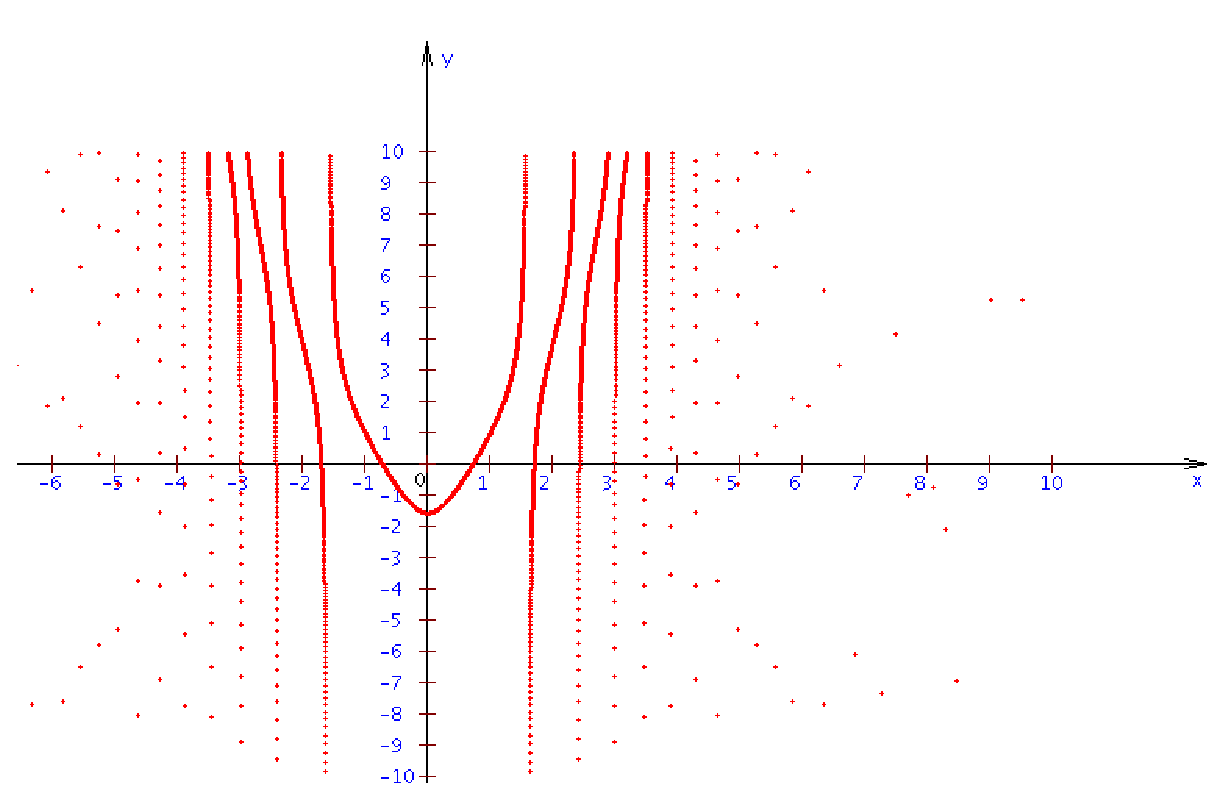
\includegraphics[scale=0.45]{pictures/3_1}
  \caption{График функции $f=x^2+\tg(x^2-1)$}
  \label{3_1}
\end{figure}

\eject

Чтобы получить графики нескольких функций на одном рисунке нужно список
этих функций заключить в квадратные скобки, как в следующем примере.

\underline{Пример 2. }

%enddelete

\begin{verbatim}
SPACE = R64[x, y, z];
\set2D(-10, 10, -10, 10);
f = \sin(x); 
p = \plot([f, \tg(x)]);
\end{verbatim}
%begindelete

\ex{$f=sin(x);$}{рис. \ref{3_3}.}

\begin{figure}[!h]
  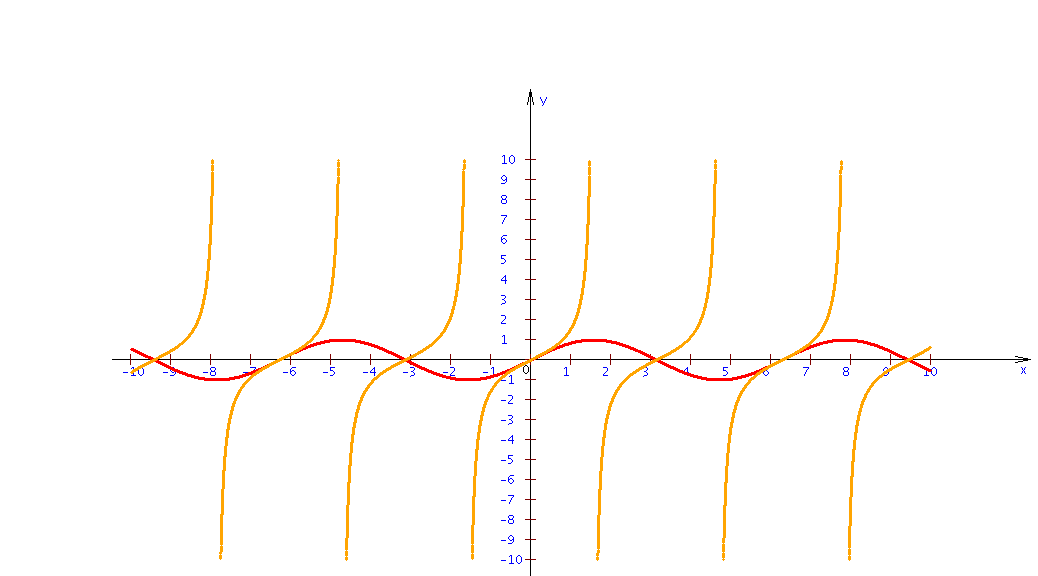
\includegraphics[width=274.6pt,height=152.38pt]{pictures/3_3}
  \caption{Графики функций $f = \sin(x)$ и $g = \tg(x)$}
  \label{3_3}
\end{figure}

\underline{Пример 3. }

%enddelete

\begin{verbatim}
SPACE = R64[x, y, z];
\set2D(-10, 10, 0, 2);
f = \unitBox(x,3); 
p = \plot(f);
\end{verbatim}
%begindelete

%\ex{$f=sin(x);$}{рис. \ref{3_3}.}

%\begin{figure}[!h]
%  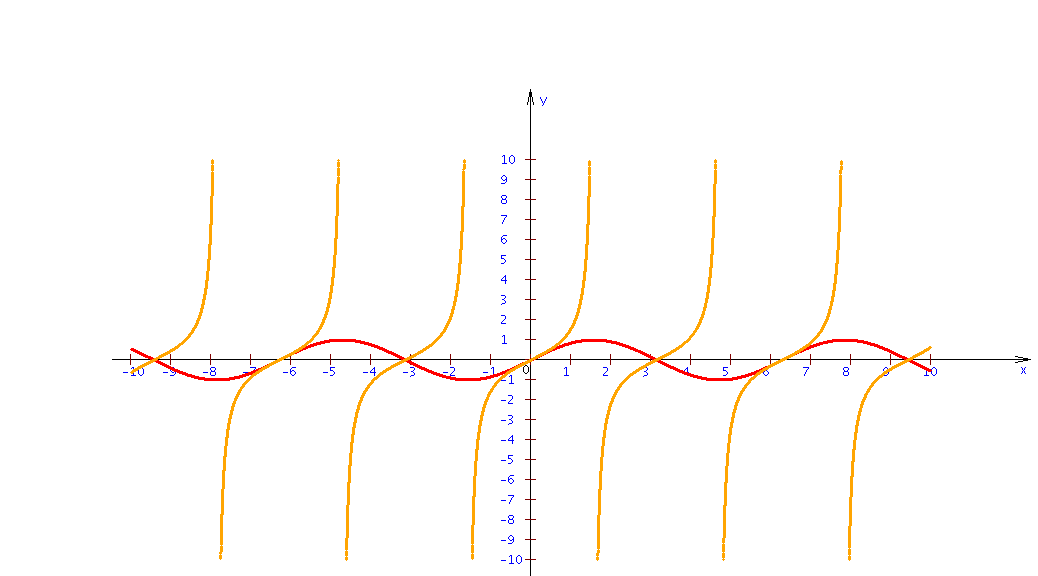
\includegraphics[width=274.6pt,height=152.38pt]{pictures/3_3}
%  \caption{Графики функций $f = \sin(x)$ и $g = \tg(x)$}
%  \label{3_3}
%\end{figure}

\underline{Пример 4. }

%enddelete

\begin{verbatim}
SPACE = R64[x, a, b, c];
\set2D(0, 2\pi, 0, 2);
\plot(a\sin(bx) + c);
\end{verbatim}

%begindelete

%  \ex{$f=sin(x);$}{pict. \ref{3_3}. }
% 
% \begin{figure}[!h]
%   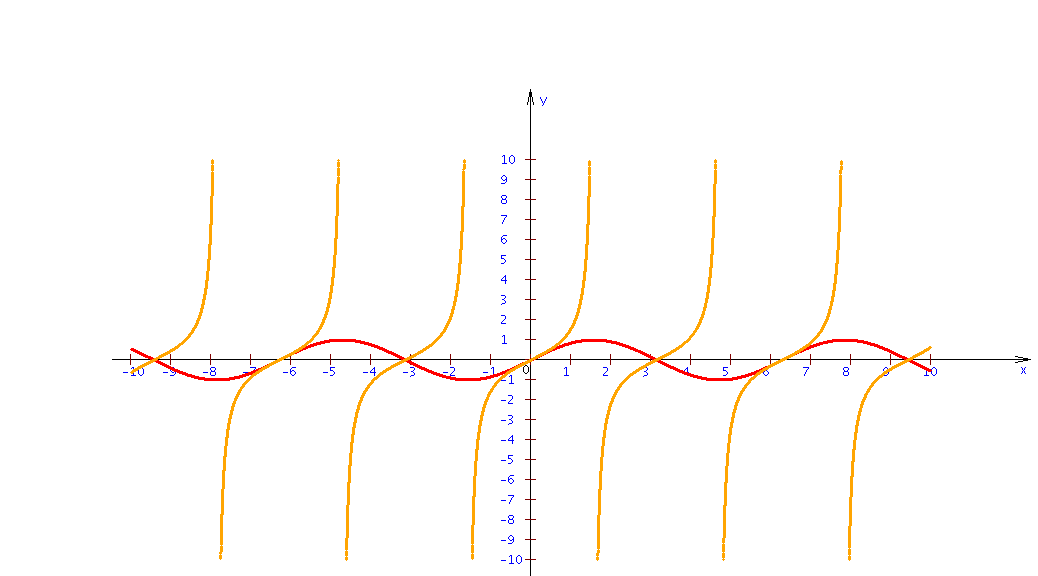
\includegraphics[width=274.6pt,height=152.38pt]{pictures/3_3}
%   \caption{Графики функций $f = \sin(x)$ и $g = \tg(x)$}
%   \label{3_3}
% \end{figure}
%enddelete

%begindelete
\underline{Пример 5. }
%enddelete
\vspace*{-2mm}
\begin{verbatim}
SPACE = R64[x, y, z];
\set2D(-10, 10, -10, 10,'a','b','title');
f = x^2; 
p = \plot(f);
\end{verbatim}
\vspace*{-2mm}

%begindelete
\underline{Пример 6. }
%enddelete
\vspace*{-2mm}
\begin{verbatim}
SPACE = R64[x, y, z];
\set2D(-10, 10, -10, 10);
f = x; 
p = \plot(f,'dash');
\end{verbatim}
\vspace*{-2mm}

%begindelete
\underline{Пример 7. }
%enddelete
\vspace*{-2mm}
\begin{verbatim}
SPACE = R64[x, y, z]; 
f = x; 
p = \plot(f,[-5,5],'arrow');
\end{verbatim}
\vspace*{-2mm}

%begindelete
\underline{Пример 8. }
%enddelete
\vspace*{-2mm}
\begin{verbatim}
SPACE = R64[x, y, z]; 
\set2D(-10, 10, -10, 10);
\plot([x,-x],'arrow');
\end{verbatim}
\vspace*{-2mm}

%begindelete
Для построения графика функции во времени с изменением параметров необходимо указать количество кадров - (например установим: frames = 5) (см. Рис.1.)

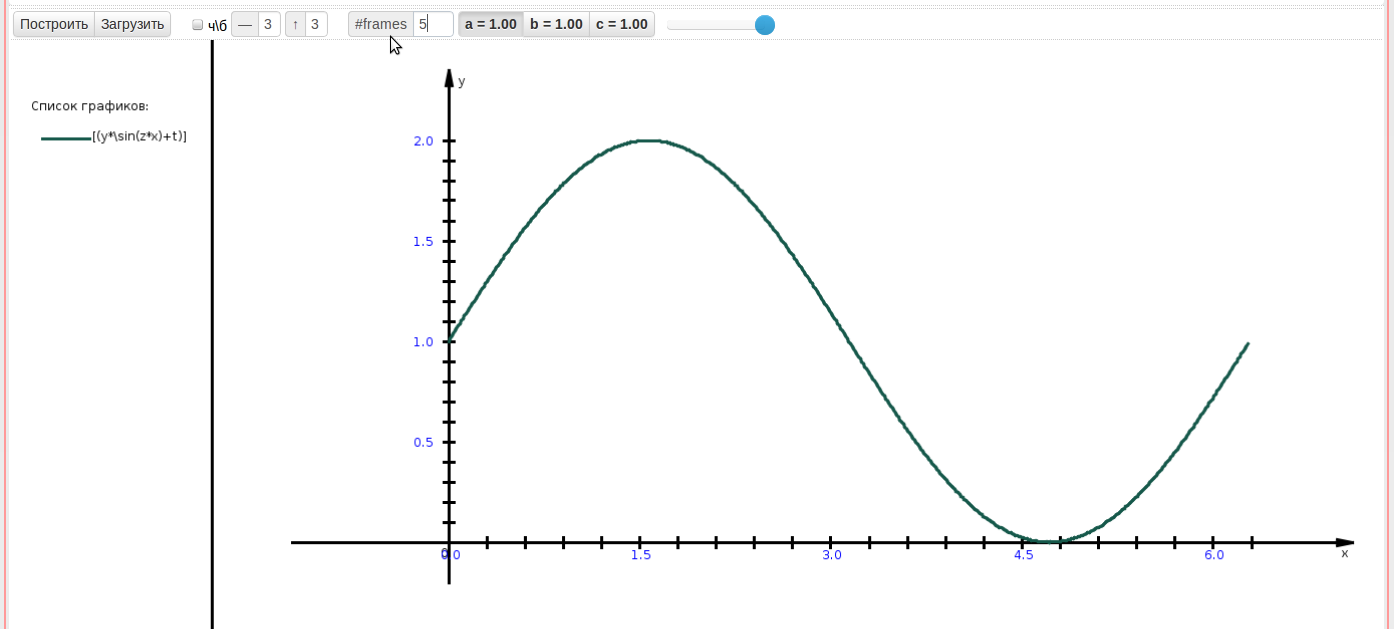
\includegraphics[scale=0.35]{pictures/2_9}

Для изменения параметров используйте ползунок - (например установим: a = 0.2, b = 0.4, c = 0.6) (см. Рис.2.)

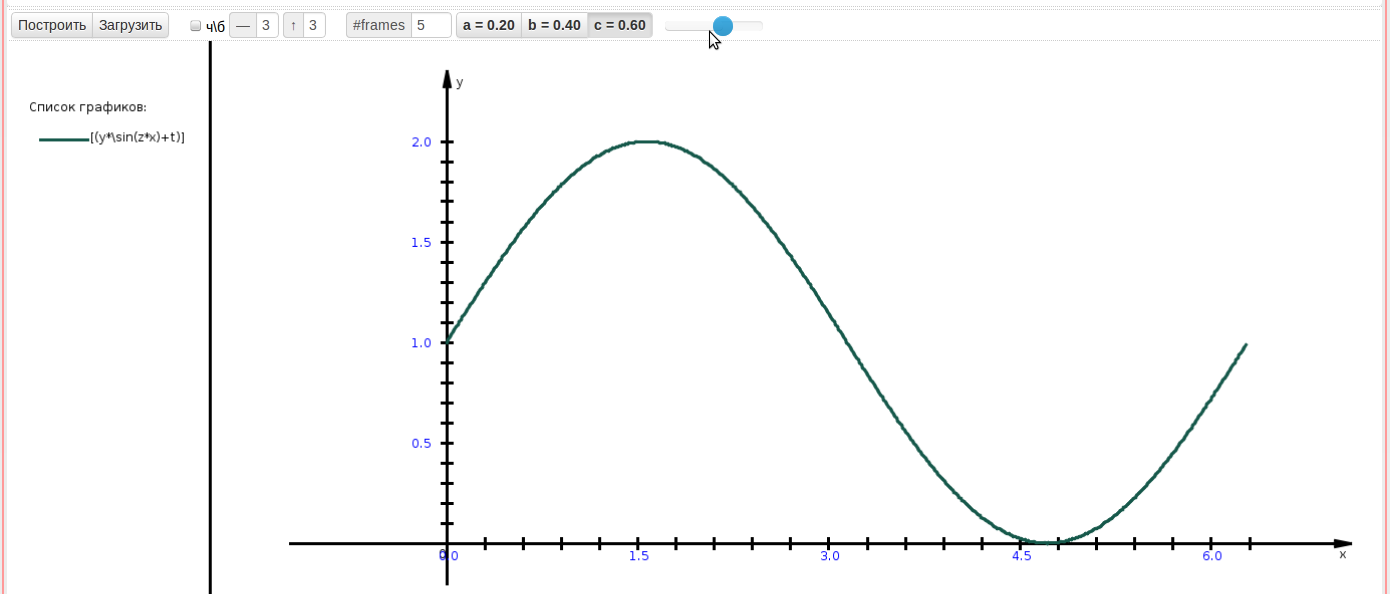
\includegraphics[scale=0.35]{pictures/2_10}

Для построения графика нажимаем кнопку - 'Построить' (см. Рис.3.)

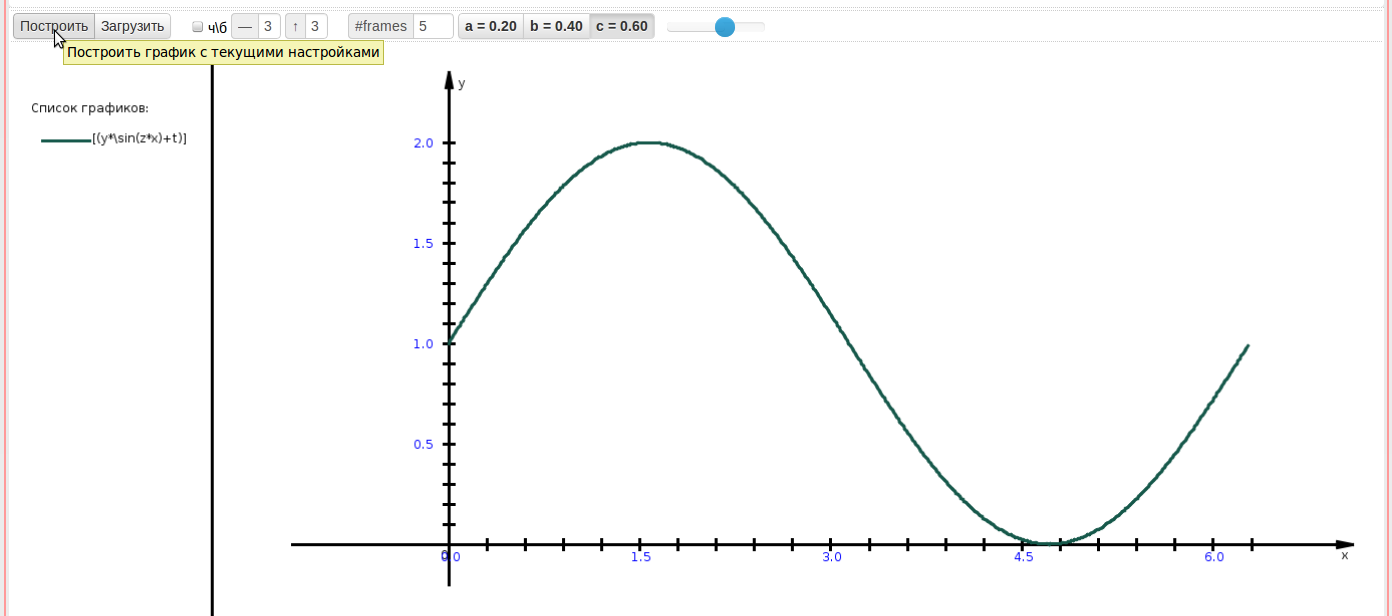
\includegraphics[scale=0.35]{pictures/2_11}

В результате получаем график.(см. Рис.4.)

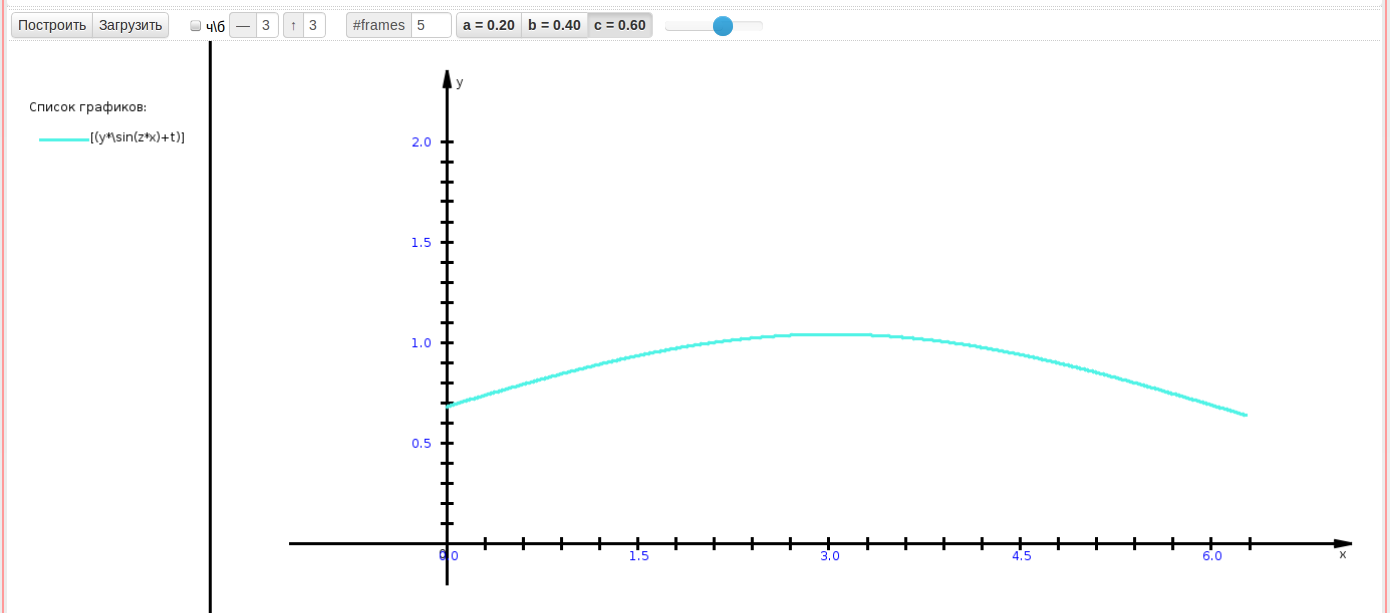
\includegraphics[scale=0.35]{pictures/2_12}

%enddelete

\subsection{Функции, заданные параметрически}
Для построения графиков функций, которые заданы параметрически,  необходимо выполнить команду 
\comm{paramPlot}{([f, g], [t0, t1])}, 
где $f = x(t)$, $g = y(t)$~--- функции,  заданная параметрически, 
$[t0, t1]$~--- интервал значений для изменения параметра. 
Другой вариант команды: \comm{paramPlot}{([f, g], [t0, t1], 'options')}, где $[t0, t1]$~--- интервал значений для изменения параметра, 
$'options'$~--- принимает следующие значения:\\
1)$'dash'$~--- график будет изображен пунктиром;\\ 
2)$'arrow'$~---  последняя точка графика будет нарисована со стрелкой;\\
3)$'dashAndArrow'$~--- график будет изображен пунктиром и последняя точка графика будет нарисована со стрелкой.\\


%begindelete
\underline{Пример 1. }


\nopagebreak
%enddelete
\vspace*{-2mm}
\begin{verbatim}
SPACE = R64[x, y, z];
g = \sin(x); 
k = \cos(x); 
f = \paramPlot([g, k], [0, 2\pi]);
\end{verbatim}
\vspace*{-2mm}

%begindelete
\ex{$g=sin(x); k=cos(x);$}{рис. \ref{3_4}.}
\begin{figure}[h!]
 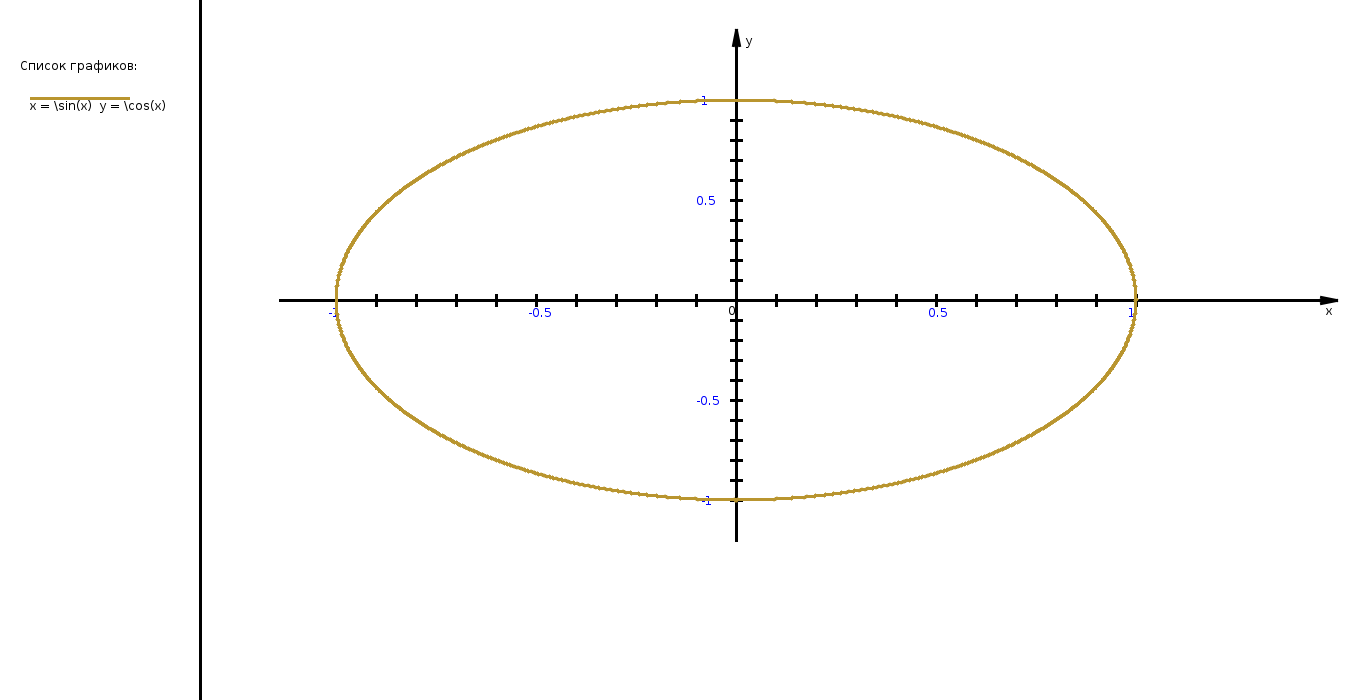
\includegraphics[scale=0.26]{pictures/2_1}
\vspace*{-10mm}
\caption{График функции, заданной параметрически}
\label{3_4}
\end{figure}
%enddelete


%begindelete
\eject
\underline{Пример 2. }


%enddelete
\vspace*{-2mm}
\begin{verbatim}
SPACE = R64[x, y, z];
g = x\sin(x);
k = x\cos(x);
f = \paramPlot([g, k], [0, 5\pi]);
\end{verbatim}
\vspace*{-2mm}

%begindelete
\ex{$g=x\sin(x); k=x\cos(x);$}{рис. \ref{2_2}.}
\begin{figure}[h!]
 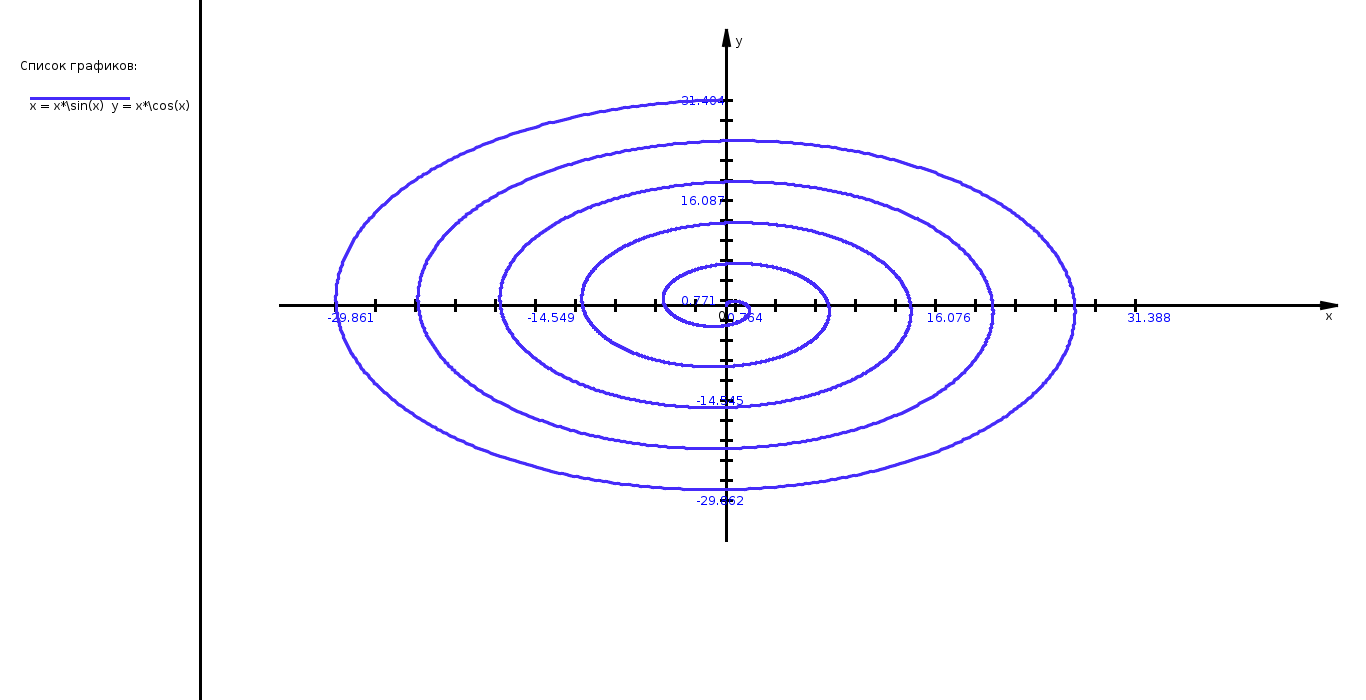
\includegraphics[scale=0.3]{pictures/2_2}
\vspace*{-10mm}
\caption{График функции, заданной параметрически}
\label{2_2}
\end{figure}



\underline{Пример 3. }

%enddelete

\vspace*{-2mm}
\begin{verbatim}
SPACE = R64[x, y, z];
g = 2\cos(x)+\cos(2x); 
k = 2\sin(x)-\sin(2x);
f = \paramPlot([g, k], [0, 2\pi]);
\end{verbatim}
\vspace*{-2mm}

%begindelete
\ex{$g=2\cos(x)+\cos(2x); k= 2\sin(x)-\sin(2x);$}{рис. \ref{2_3}.}
\begin{figure}[h!]
 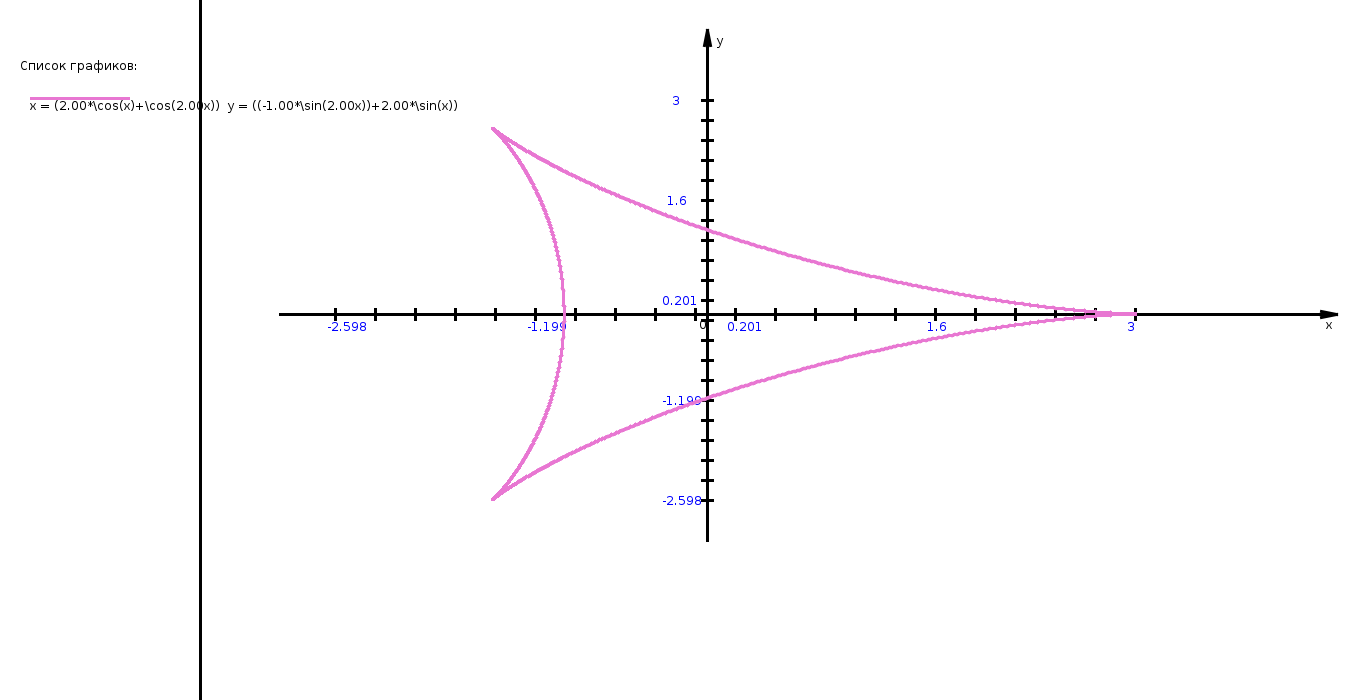
\includegraphics[scale=0.3]{pictures/2_3}
\vspace*{-10mm}
\caption{График функции, заданной параметрически}
\label{2_3}
\end{figure}

\eject
\underline{Пример 4. }


%enddelete

\vspace*{-2mm}
\begin{verbatim}
SPACE = R64[x, y, z];
g = 2\sin(x)^3; 
k = 2\cos(x)^3;
f = \paramPlot([g, k], [0, 2\pi]);
\end{verbatim}
\vspace*{-2mm}


%begindelete
\ex{$g=2\sin(x)^3; k= 2\cos^3(x)$}{рис. \ref{2_4}.}
\begin{figure}[h!]
 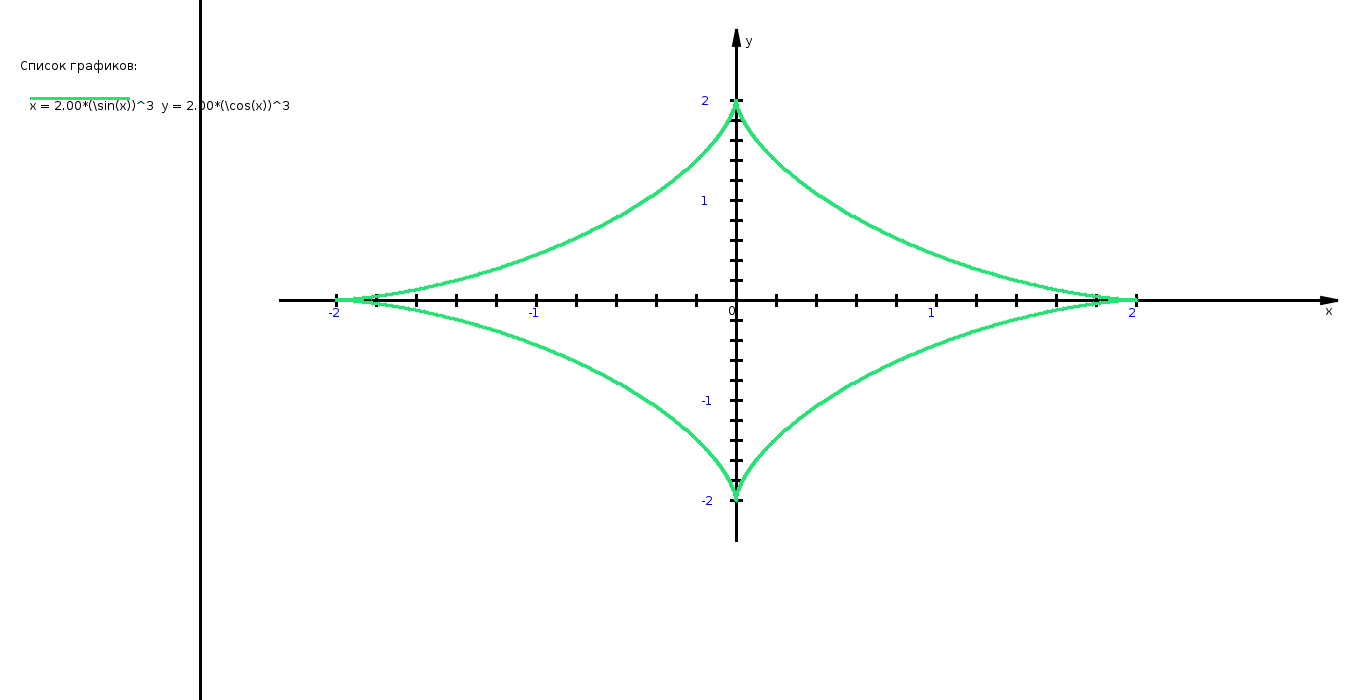
\includegraphics[scale=0.3]{pictures/2_4}
\vspace*{-10mm}
\caption{График функции, заданной параметрически}
\label{2_4}
\end{figure}



\underline{Пример 5. }
%enddelete

\vspace*{-2mm}
\begin{verbatim}
SPACE = R64[x, y, z];
g = (1+\cos(x))\cos(x); 
k = (1+\cos(x))\sin(x);
f = \paramPlot([g, k], [0, 2\pi]);
\end{verbatim}
\vspace*{-2mm}

%begindelete
\ex{$g=(1+\cos(x))\cos(x);k= (1+\cos(x))\sin(x);$}{рис. \ref{2_5}.}
\begin{figure}[h!]
 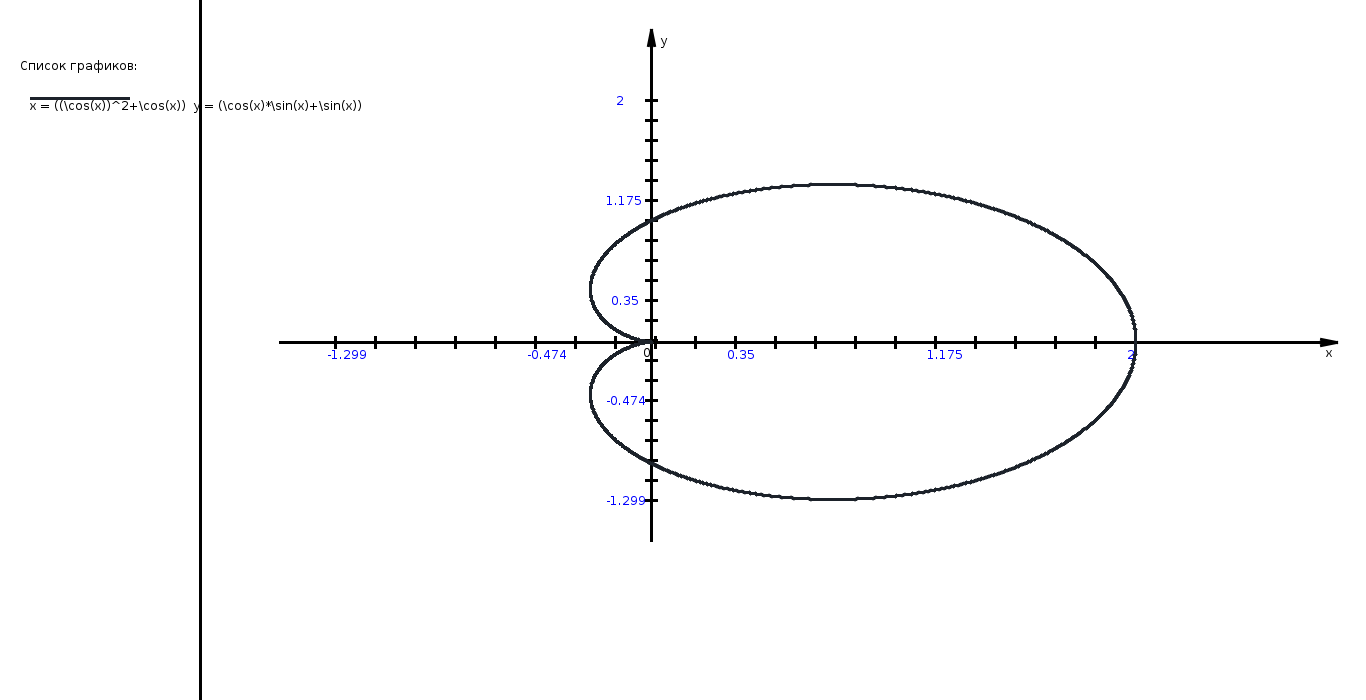
\includegraphics[scale=0.3]{pictures/2_5}
\vspace*{-10mm}
\caption{График функции, заданной параметрически}
\label{2_5}
\end{figure}

\eject
\underline{Пример 6. }
%enddelete


\vspace*{-2mm}
\begin{verbatim}
SPACE = R64[x, y, z];
g = \sin(x)(\exp(\cos(x))-2\cos(4x)+\sin(x/12)^5);
k = \cos(x)(\exp(\cos(x))-2\cos(4x)+\sin(x/12)^5);
f = \paramPlot([g, k], [0, 12\pi]);
\end{verbatim}
\vspace*{-2mm}


%begindelete
\ex{$g=\sin(x)(\exp(\cos(x))-2\cos(4x)+\sin^5(x/12));$\\
\hspace*{4mm} $k= \cos(x)(\exp(\cos(x))-2\cos(4x)+\sin^5(x/12));$}{рис. \ref{2_6}.}
\begin{figure}[h!]
 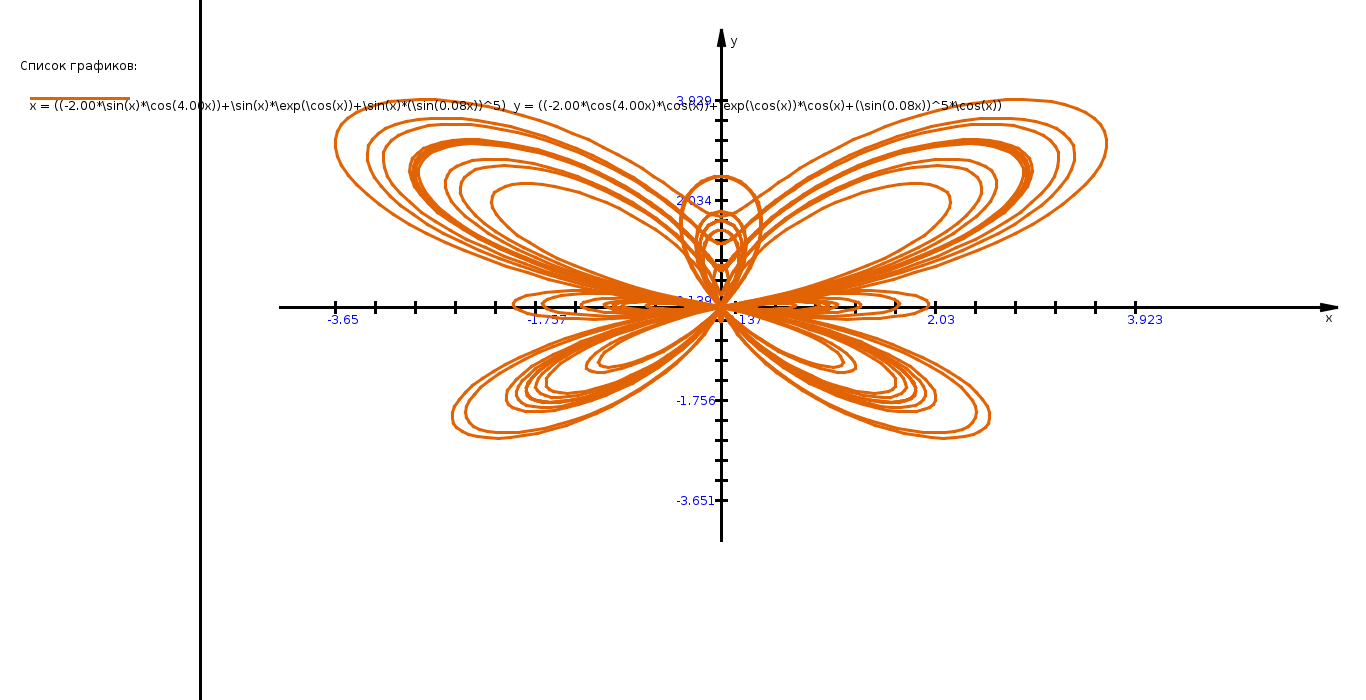
\includegraphics[scale=0.3]{pictures/2_6}
\vspace*{-10mm}
\caption{График функции, заданной параметрически}
\label{2_6}
\end{figure}
 

\eject
\underline{Пример 7. }
%enddelete


\vspace*{-2mm}
\begin{verbatim}
SPACE = R64[x, y, z];
\set2D('','','','','x(t)','y(t)','paramPlot');
g = \sin(x)(\exp(\cos(x))-2\cos(4x)+\sin(x/12)^5);
k = \cos(x)(\exp(\cos(x))-2\cos(4x)+\sin(x/12)^5);
f = \paramPlot([g, k], [0, 12\pi]);
\end{verbatim}
\vspace*{-2mm}

%begindelete
\eject
\underline{Пример 8. }
%enddelete

\vspace*{-2mm}
\begin{verbatim}
SPACE = R64[x, y, z];
g = \sin(x); 
k = \cos(x); 
f = \paramPlot([g, k], [0, 2\pi],'dashAndArrow');
\end{verbatim}
\vspace*{-2mm}


\subsection{Функции, которые заданы таблицей значений}

Для построения графиков функций, заданных табличными значениями, необходимо выполнить команду:
\comm{tablePlot}{([[x_{1},\ldots, x_{n}],[y_{11},\ldots,a_{1n}],\ldots,[y_{k1},\ldots,a_{kn}]])}
Другой вариант команды:
\comm{tablePlot}{([[x_{1},\ldots, x_{n}],[y_{11},\ldots,a_{1n}],\ldots,[y_{k1},\ldots,a_{kn}]], 'options')}
,где $'options'$~--- принимает следующие значения:\\
1)$'dash'$~--- график будет изображен пунктиром;\\ 
2)$'arrow'$~---  последняя точка графика будет нарисована со стрелкой;\\
3)$'dashAndArrow'$~--- график будет изображен пунктиром и последняя точка графика будет нарисована со стрелкой.

%begindelete
\underline{Пример 1.}
 
 \vspace*{-2mm}
%enddelete

 \begin{verbatim}
SPACE = R64[x, y, z];
 \tablePlot(
   [
     [0, 1, 2, 3, 4, 5],
     [0, 1, 4, 9, 16, 25],
     [0, -1, -2, -3, -4, -5],
     [0, 4, 8, 12, 16, 20]
   ]);
 \end{verbatim}

 %begindelete
\ex{}{рис. \ref{2_7}.}
\begin{figure}[!h]
 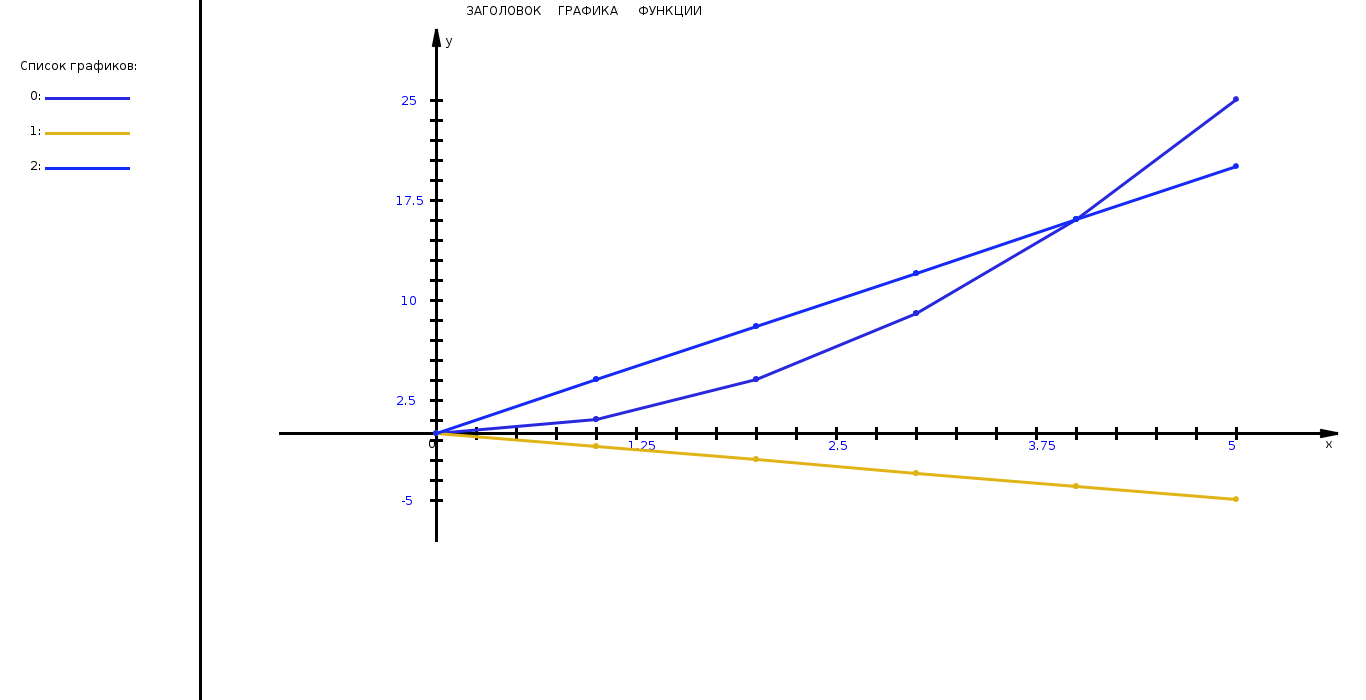
\includegraphics[scale=0.25]{pictures/2_7}
\vspace*{-10mm}
\caption{График функции, заданной таблицей значений}
\label{2_7}
\end{figure}


\underline{Пример 2.}
 %enddelete

 \vspace*{-2mm}
 \begin{verbatim}
SPACE=R64[x]; 
\set2D(-1,5,-10,10);
"Пусть задана табличная функция:" 
A=[[0, 1, 2, 3,  4, 5],    [3, 0, 4, 10, 5, 10]]; t=\table(A);
"Аппроксимируем эту функцию полиномом 4-й степени:" p=\approx(t,4);
"Построим график полинома:" P=\plot(p,[1,5]);
"Построим график табличной функции:" T=\tablePlot(t);
"Построим оба графика в одной системе координат:" \showPlots([P,T]);
\print(p);
 \end{verbatim}

%begindelete
\ex{}{$0.54x^4-5.64x^3+18.38x^2-17.28x+3.17$\\
\hspace*{4mm} рис. \ref{2_8}.}
\begin{figure}[!h]
 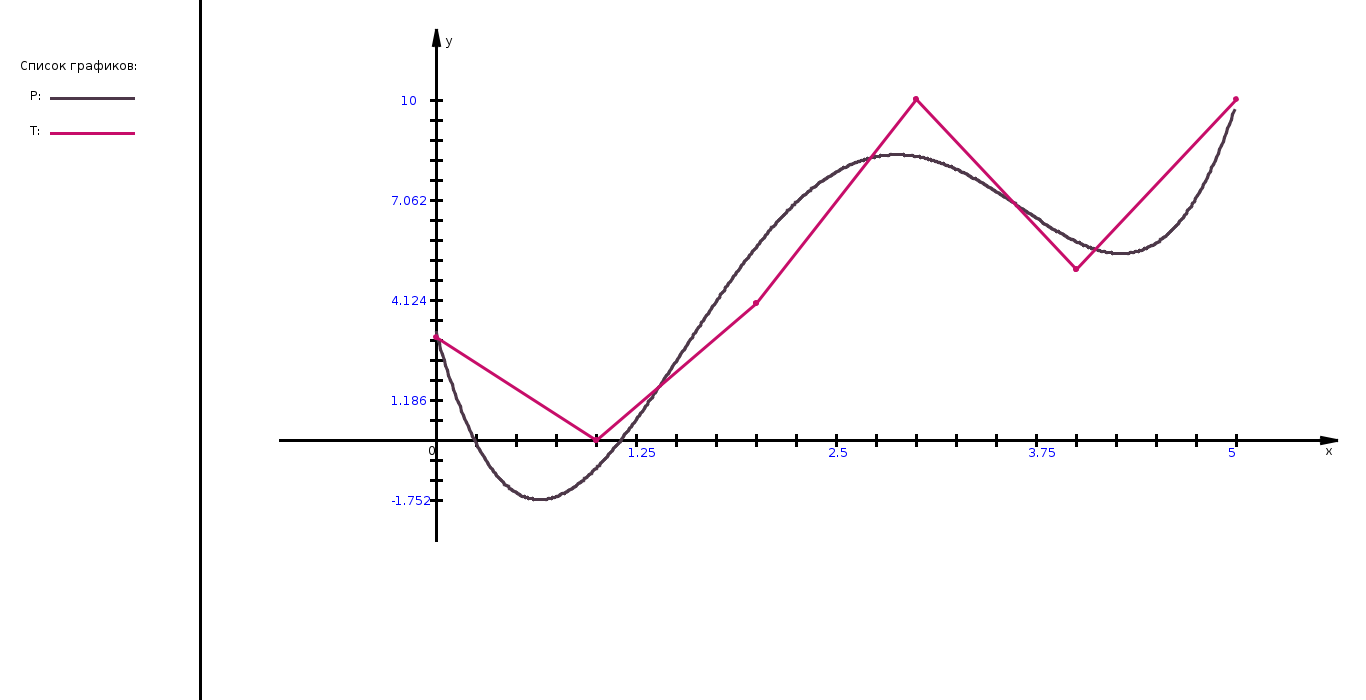
\includegraphics[scale=0.25]{pictures/2_8}
\vspace*{-10mm}
\caption{График аппроксимации функции, заданной таблицей значений}
\label{2_8}
\end{figure}
%enddelete

%begindelete
\underline{Пример 3.}
 
 \vspace*{-2mm}
%enddelete

 \begin{verbatim}
SPACE = R64[x, y, z];
\set2D(-10, 10, -10, 10, '','', 'Header of Graphics');
 \tablePlot(
   [[-3, -6, -6, -3, 3, 6, 6, 3, -3],
    [6, 3, -3, -6, -6, -3, 3, 6, 6]]);
 \end{verbatim}

%begindelete
\underline{Пример 4.}
 
 \vspace*{-2mm}
%enddelete

 \begin{verbatim}
SPACE = R64[x, y, z];
 \tablePlot(
   [[-3, -6, -6, -3, 3, 6, 6, 3, -3],
    [6, 3, -3, -6, -6, -3, 3, 6, 6]],'arrow');
 \end{verbatim}

%begindelete
\underline{Пример 5.}
 
 \vspace*{-2mm}
%enddelete

 \begin{verbatim}
SPACE = R64[x, y, z];
 \tablePlot(
   [[-3, -6, -6, -3, 3, 6, 6, 3, -3],
    [6, 3, -3, -6, -6, -3, 3, 6, 6]], 'dash');
 \end{verbatim}

%begindelete
\underline{Пример 6.}
 
 \vspace*{-2mm}
%enddelete

 \begin{verbatim}
SPACE = R64[x, y, z];
 \tablePlot(
   [[-3, -6, -6, -3, 3, 6, 6, 3, -3],
    [6, 3, -3, -6, -6, -3, 3, 6, 6]], 'dashAndArrow');
 \end{verbatim}

\subsection{Функции, которые заданы таблицей значений по точкам}
Для построения графиков функций по точкам, заданных табличными значениями, необходимо выполнить команду: 
\comm{pointsPlot}{([[x_{1},\ldots, x_{n}],[y_{1},\ldots,y_{n}]], [s_{1},\ldots,s_{n}], [kv_{1},\ldots,kv_{n}], [kg_{1},\ldots,kg_{n}])},\\
где $s_{n}$~--- подпись точки, $kv_{n}$~--- коэффициент поворота вокруг точки (принимает значения от 0 до 7, и означает поворот на ($kv_{n}$ * 45) градусов), 
$kg_{n}$~--- коэффициент смещения вдоль оси $OX$ (если отрицательный то смещение происходит влево).
Сокращенные варианты команды:
\comm{pointsPlot}{([[x_{1},\ldots, x_{n}],[y_{1},\ldots,y_{n}]], [s_{1},\ldots,s_{n}])}
или
\comm{pointsPlot}{([[x_{1},\ldots, x_{n}],[y_{1},\ldots,y_{n}]], [s_{1},\ldots,s_{n}], [kv_{1},\ldots,kv_{n}])}
или
\comm{pointsPlot}{([[x_{1},\ldots, x_{n}],[y_{1},\ldots,y_{n}]], [s_{1},\ldots,s_{n}], [kv_{1},\ldots,kv_{n}], [kg_{1},\ldots,kg_{n}])}.

%begindelete
\underline{Пример 1.}
 
 \vspace*{-2mm}
%enddelete

 \begin{verbatim}
\set2D(-10, 10, -10, 10);
\pointsPlot(
   [[0, 1, 2],
     [0, 1, 4]],['a','b','c']);
 \end{verbatim}

%begindelete
\underline{Пример 2.}
 
 \vspace*{-2mm}
%enddelete

 \begin{verbatim}
 \pointsPlot(
   [
     [0, 1, 2],
     [0, 1, 4]],['a','b','c'],[0,2,4]);
 \end{verbatim}

%begindelete
\underline{Пример 3.}
 
 \vspace*{-2mm}
%enddelete

 \begin{verbatim}
 \pointsPlot(
   [
     [0, 1, 2],
     [0, 1, 4]],['a','b','c'],[0,2,4],[0,-5,5]);
 \end{verbatim}

%begindelete
\underline{Пример 4.}
 
 \vspace*{-2mm}
%enddelete

 \begin{verbatim}
 \pointsPlot(
   [
     [0, 1, 2],
     [0, 1, 4]]);
 \end{verbatim}

%begindelete
\underline{Пример 5.}
 
 \vspace*{-2mm}
%enddelete

 \begin{verbatim}
SPACE = R64[x, y, z];
f1=\tablePlot([[1, 1], [1, 5]]);
f2=\tablePlot([[1, 5], [1, 1]]);
f3=\tablePlot([[5, 5], [1, 5]]);
f4=\tablePlot([[1, 5], [5, 5]]);
f5=\pointsPlot([[1, 1, 5, 5],[1, 5, 5, 1]],['A','B','C','D'],[6,0,0,2]);
\showPlots([f1, f2, f3, f4, f5]);
 \end{verbatim}

%begindelete
\underline{Пример 6.}
 
 \vspace*{-2mm}
%enddelete

 \begin{verbatim}
SPACE = R64[x, y, z];
f1=\tablePlot([[1, 1], [1, 5]]);
f2=\tablePlot([[1, 5], [1, 1]]);
f3=\tablePlot([[5, 5], [1, 5]]);
f4=\tablePlot([[1, 5], [5, 5]]);
f5=\pointsPlot([[1, 1, 5, 5],[1, 5, 5, 1]],['A','B','C','D'],[6,0,0,2]);
\showPlots([f1, f2, f3, f4, f5],'noAxes');
 \end{verbatim}

\subsection{Построение разных графиков функций в одной системе координат}
Для построения графиков функций,  заданных разными способами,  необходимо сначала построить график каждой функции,  а затем выполнить команду
\comm{showPlots}{([f_1, f_2, \ldots, f_n])}.
Другие варианты команды:
\comm{showPlots}{([f1, f2, f3, f4], 'noAxes')}, где 'noAxes'~--- параметр, указывающий на изображение графика без осей.
или
\comm{showPlots}{([f1, f2, f3, f4], 'lattice')}, где 'lattice'~--- параметр, указывающий на изображение графика c решеткой.

%begindelete
\underline{Пример 1.}
 
 \vspace*{-2mm}
%enddelete

\begin{verbatim}
SPACE = R64[x, y, z];
\set2D(-20, 20, -20, 20);
f1 = \plot(\tg(x));
f2 = \tablePlot([[0, 1, 4, 9, 16, 25], [0, 1, 2, 3, 4, 5]]);
f3 = \paramPlot([\sin(x), \cos(x)], [-10, 10]);
f4=\tablePlot([[0, 1, 4, 9, 16, 25], [0, -1, -2, -3, -4, -5]]);
\showPlots([f1, f2, f3, f4]);
\end{verbatim}
%begindelete
\ex{}{рис. \ref{3_6}.}
\begin{figure}[!ht]
 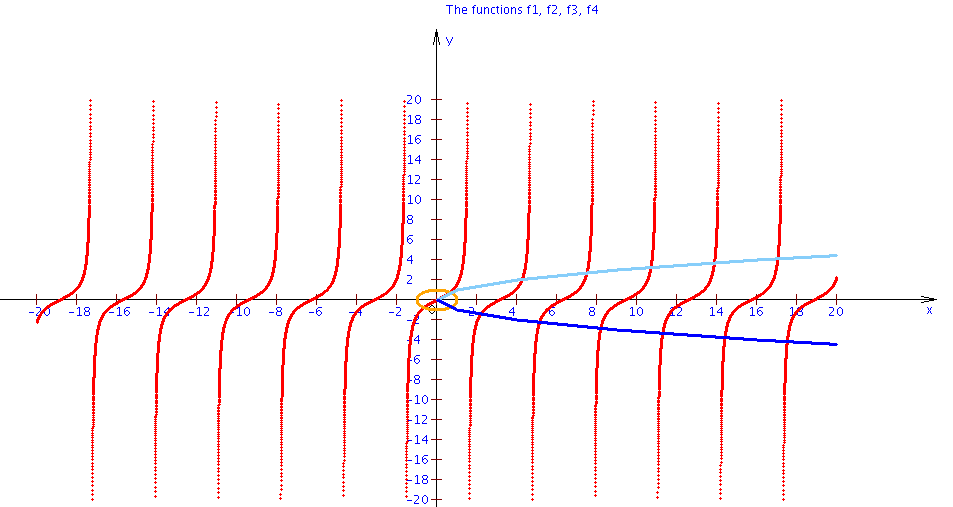
\includegraphics[scale=0.6]{pictures/3_6}
\caption{Графики функций,  заданных разными способами}
\label{3_6}
\end{figure}
%enddelete

%begindelete
\underline{Пример 2.}
 
 \vspace*{-2mm}
%enddelete

 \begin{verbatim}
p1=\tablePlot([[-1, -3, 3, 3, -3, -3],[4, 3, 3, -3 , -3, 3]]);
p2=\tablePlot([[5, 5, 3, 3, 5, -1],[4, -2, -3, 3, 4, 4]]);
p3=\tablePlot([[-3, -1, -1],[-3, -2, 4]], 'dash');
p4=\tablePlot([[-1, 5],[-2, -2]], 'dash');
\showPlots([p1,p2,p3,p4], 'noAxes');
 \end{verbatim}

%begindelete
\underline{Пример 3.}
 
 \vspace*{-2mm}
%enddelete

 \begin{verbatim}
p1=\tablePlot([[-1, -3, 3, 3, -3, -3],[4, 3, 3, -3, -3, 3]]);
p1p=\pointsPlot([[-1, -3, 3, 3, -3],[4, 3, 3, -3 , -3]],
['F','B','C','D','A'],[0,0,0,4,4]);
p2=\tablePlot([[5, 5, 3, 3, 5, -1],[4, -2, -3, 3, 4, 4]]);
p3=\tablePlot([[-3, -1, -1],[-3, -2, 4]],'dash');
p4=\tablePlot([[-1, 5],[-2, -2]],'dash');
p2p=\pointsPlot([[5, 5, -1 ],[4, -2, -2]],['G','H','E'],[0,4,4]);
\showPlots([p1,p2,p3,p4,p1p,p2p], 'noAxes');
 \end{verbatim}


\subsection{Построение графов}
Для построения графов необходимо выполнить команду 
\comm{plotGraph}{([[a_{11},\ldots,a_{1n}],\ldots,[a_{n1},\ldots,a_{nn}]], [[x_{1},\ldots, x_{n}],[y_{1},\ldots,y_{n}]])}, 
где $[[a_{11},\ldots,a_{1n}],\ldots,[a_{n1},\ldots,a_{nn}]]$~--- матрица смежности, $[[x_{1},\ldots, x_{n}],[y_{1},\ldots,y_{n}]]$~--- матрица координат.

%begindelete
\underline{Пример 1. }

\vspace*{-2mm}
%enddelete
\begin{verbatim}
\plotGraph([[0,1,1,0,1,0],[1,0,0,1,1,0],[1,0,0,0,1,1],[0,1,0,0,0,0],
[1,1,1,0,0,1],[0,0,1,0,1,0]],[[3,2,4,1,3,5],[3,2,2,1,1,1]]);
\end{verbatim}
%begindelete
\ex{}{рис. \ref{4_1}.}
\begin{figure}[!ht]
 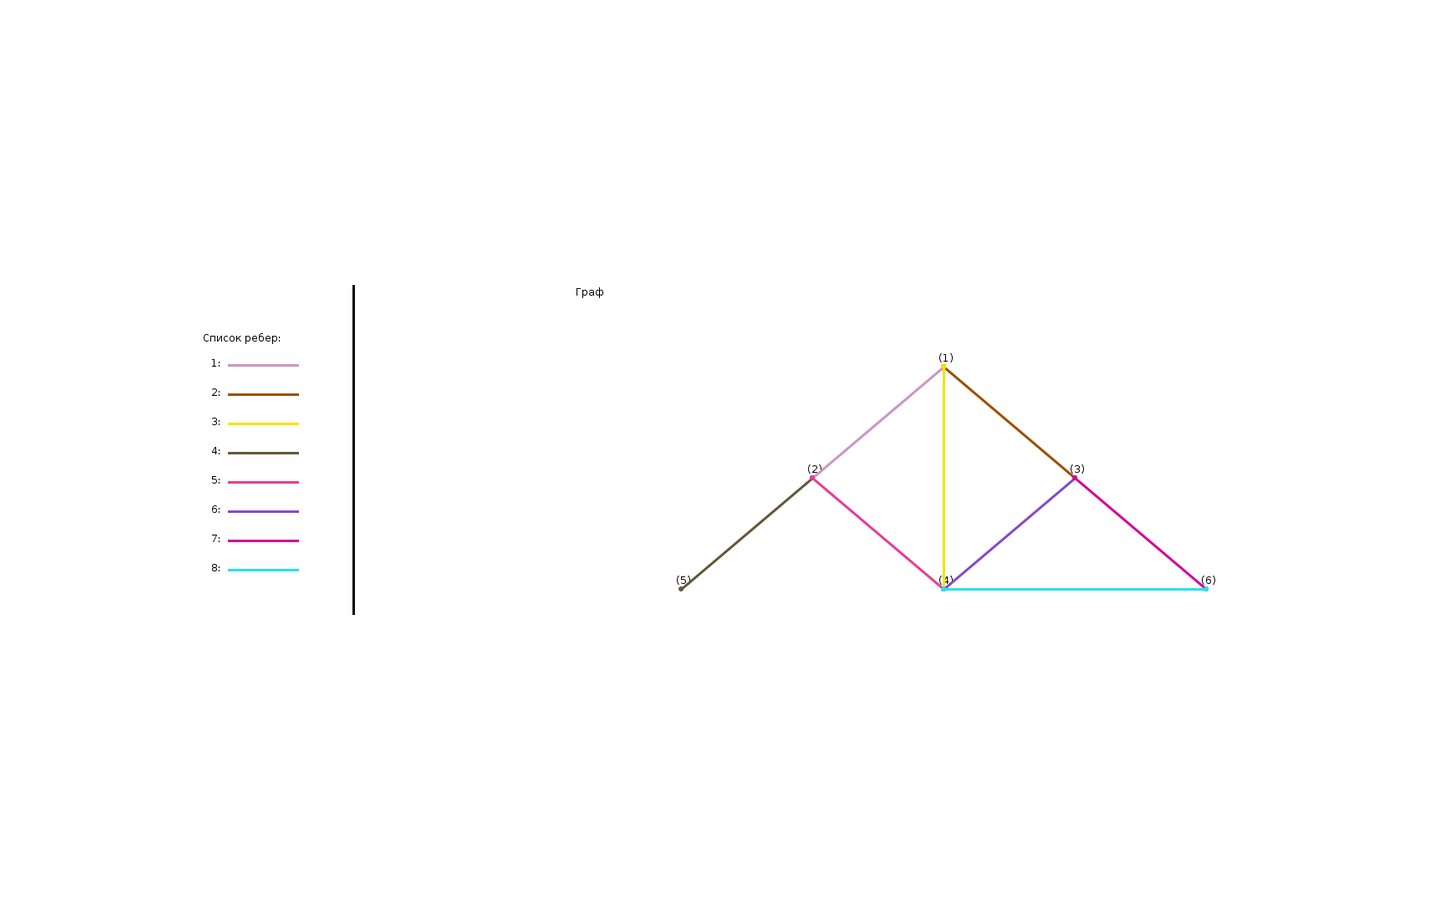
\includegraphics[scale=0.4]{pictures/4_1}
\caption{Граф}
\label{4_1}
\end{figure}
%enddelete

Кроме того, можно выполнить команду лишь с первым параметром 
\comm{plotGraph}{([[a_{11},\ldots,a_{1n}],\ldots,[a_{n1},\ldots,a_{nn}]])}, 
где $[[a_{11},\ldots,a_{1n}],\ldots,[a_{n1},\ldots,a_{nn}]]$~--- матрица смежности.

%begindelete
\underline{Пример 2. }

\vspace*{-2mm}%enddelete
\begin{verbatim}
\plotGraph([[0,1,1,0,1,0],[1,0,0,1,1,0],[1,0,0,0,1,1],[0,1,0,0,0,0],
[1,1,1,0,0,1],[0,0,1,0,1,0]]);
\end{verbatim}
%begindelete
\ex{}{рис. \ref{4_2}.}
\begin{figure}[!ht]
 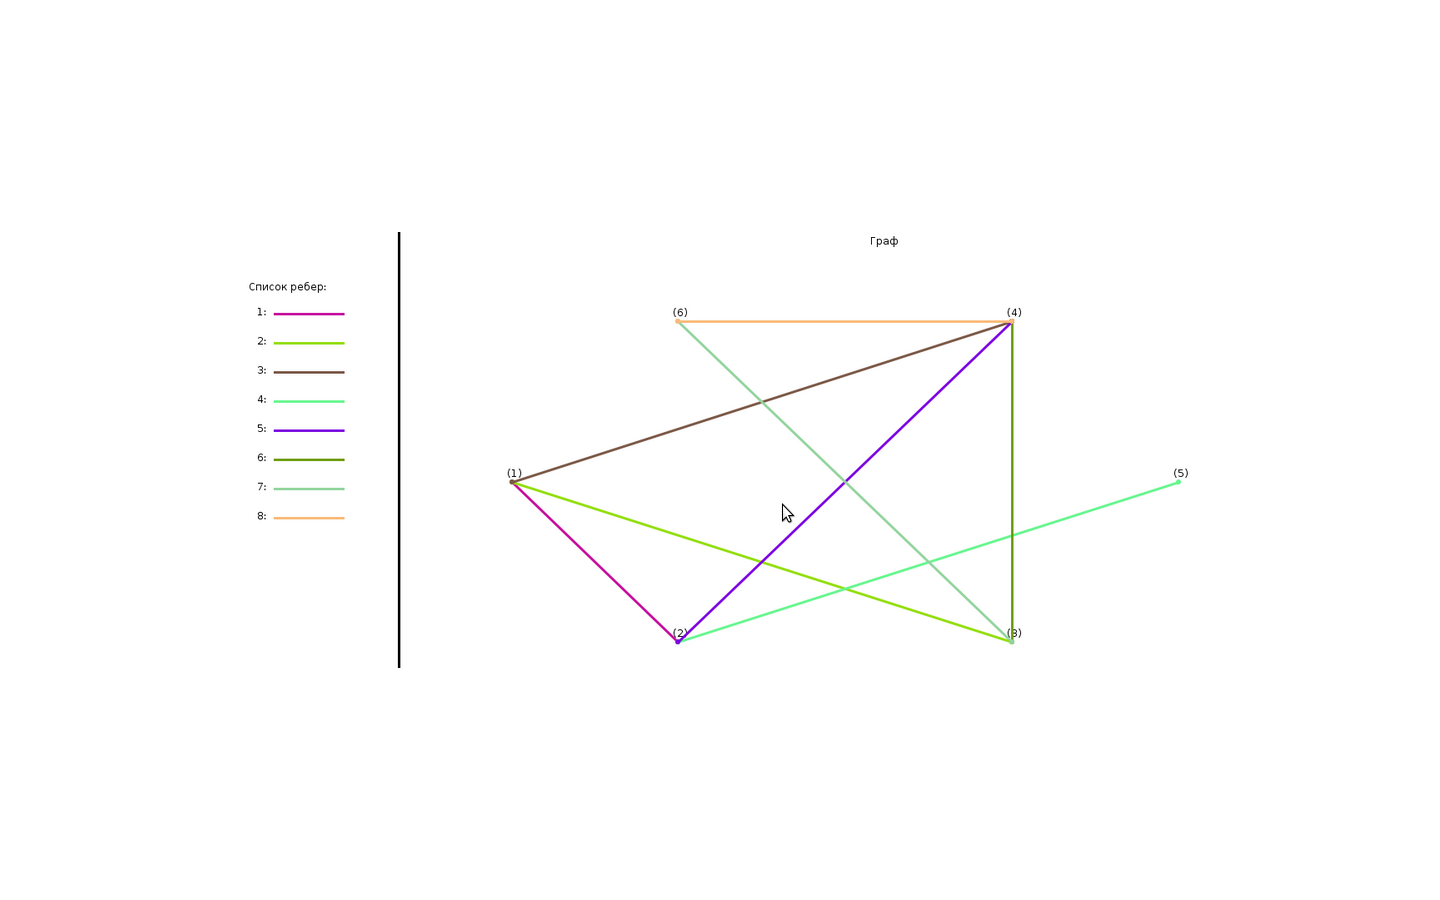
\includegraphics[scale=0.4]{pictures/4_2}
\caption{Граф}
\label{4_2}
\end{figure}
%enddelete

Можно выполнить команду с одним числовым параметром 
\comm{plotGraph}{(N)}, 
где $N$~--- количество вершин в графе.

%begindelete
\underline{Пример 3. }

\vspace*{-2mm}%enddelete
\begin{verbatim}
\plotGraph(6);
\end{verbatim}
%begindelete
\ex{}{рис. \ref{4_3}.}
\begin{figure}[!ht]
 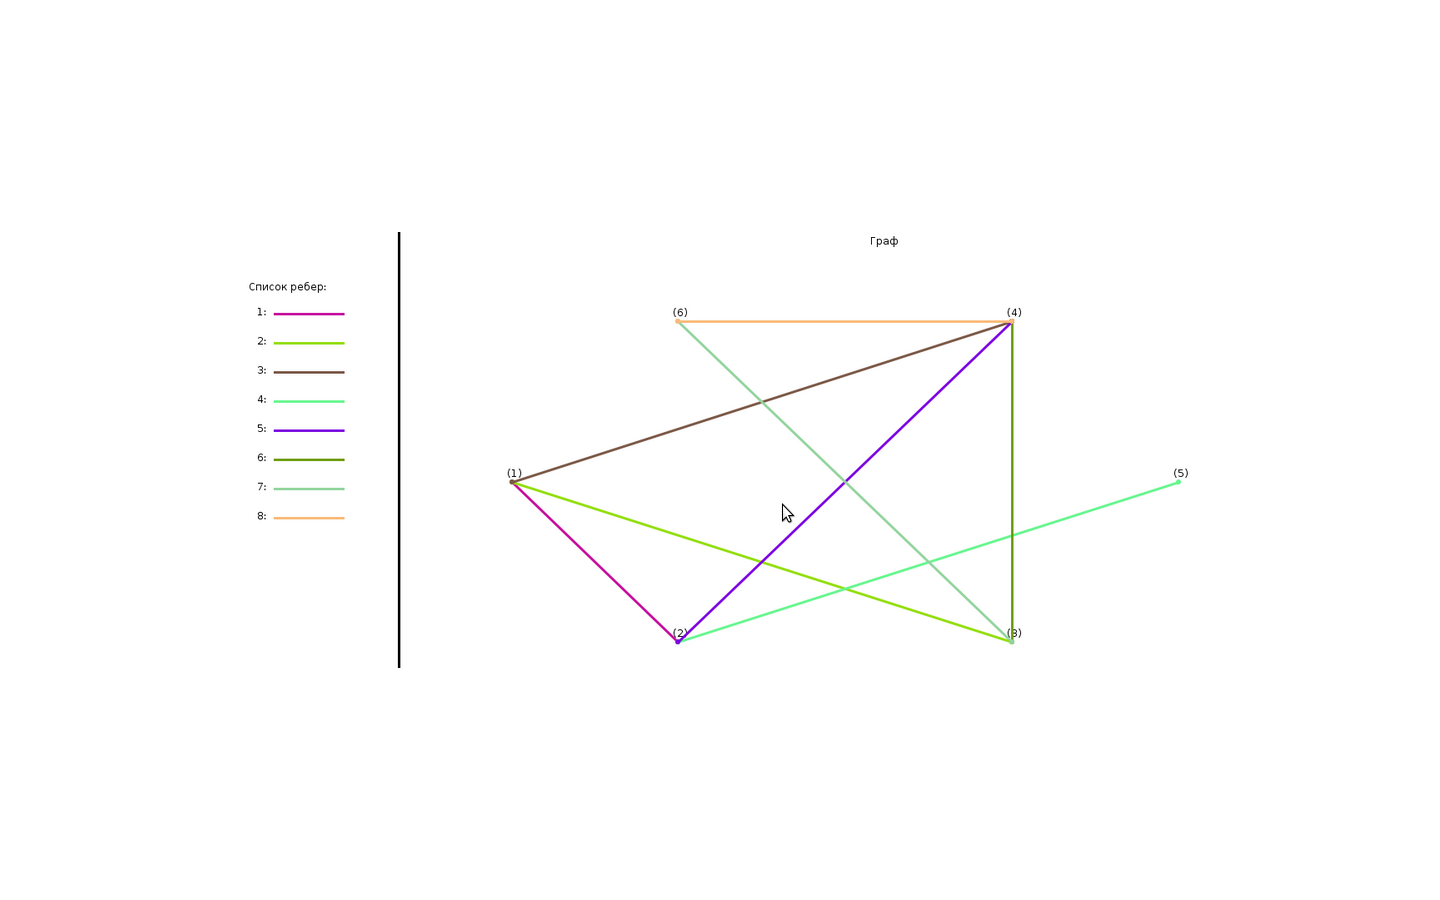
\includegraphics[scale=0.4]{pictures/4_2}
\caption{Граф}
\label{4_3}
\end{figure}
%enddelete


\subsection{Текст на графиках}
Для того, чтобы делать любые виды надписей используется функция
\comm{textPlot}{()}

Для задания одной надписи записывают в кваратных скобках
следуюшие параметры: ['str',sizeText,xCor,yCor,alpha]

  где str - это текст; sizeText - размер шрифта; xCor, yCor - координаты на экране первой буквы текста,
  alpha - угол наклона текста  (по умолчанию, если это параметр не указан, то он равен нулю). 

В одной команде можно определить сколько угоно надписей, разделяя их запятыми:\\
  \comm{textPlot}{([],[],[],...[])}.

\section{Построение 3D графиков функций}
 Mathpar позволяет строить 3D графики функций, которые заданы явно. 
 
 Для построения 3D графика функции $f=f(x, y)$ используется команда 
\comm{plot3d}{(f, [x0, x1, y0, y1])},
 где $[x0, x1]$~--- интервал по оси $OX$,  $[y0, y1]$~--- интервал по оси $OY$. 
 
Кроме того,  полученные графики можно вращать и масштабировать: увеличивать либо уменьшать. 

 Перемещение мыши с нажатой левой кнопкой приводит к вращению системы координат графика. 
 После остановки происходит перерисовка графика в новой повернутой системе координат. 
 
 Перемещение мыши с нажатой левой кнопкой и нажатой клавишей {\it Shift} приводит к изменению масштаба изображения. 
 После остановки перемещения происходит перерисовка графика в новом масштабе.  

\underline{Пример. }

\vspace*{-2mm}

\begin{verbatim}
f = x^2 / 20 + y^2 / 20;
\plot3d(f, [-20, 20, -20, 20]);
\end{verbatim}

\begin{verbatim}
\plot3d([x / 20 + y^2 / 20, x^2 / 20 + y / 20], [-20, 20, -20, 20]);
\end{verbatim}

\begin{verbatim}
SPACE = R64[x, y, a, b];
f = ax^2 / 20 + by^2 / 20;
\plot3d(f, [-20, 20, -20, 20]);
\end{verbatim}

%begindelete

Для построения графика функции во времени с изменением параметров необходимо указать количество кадров - (например установим: frames = 5) (см. Рис.1.)

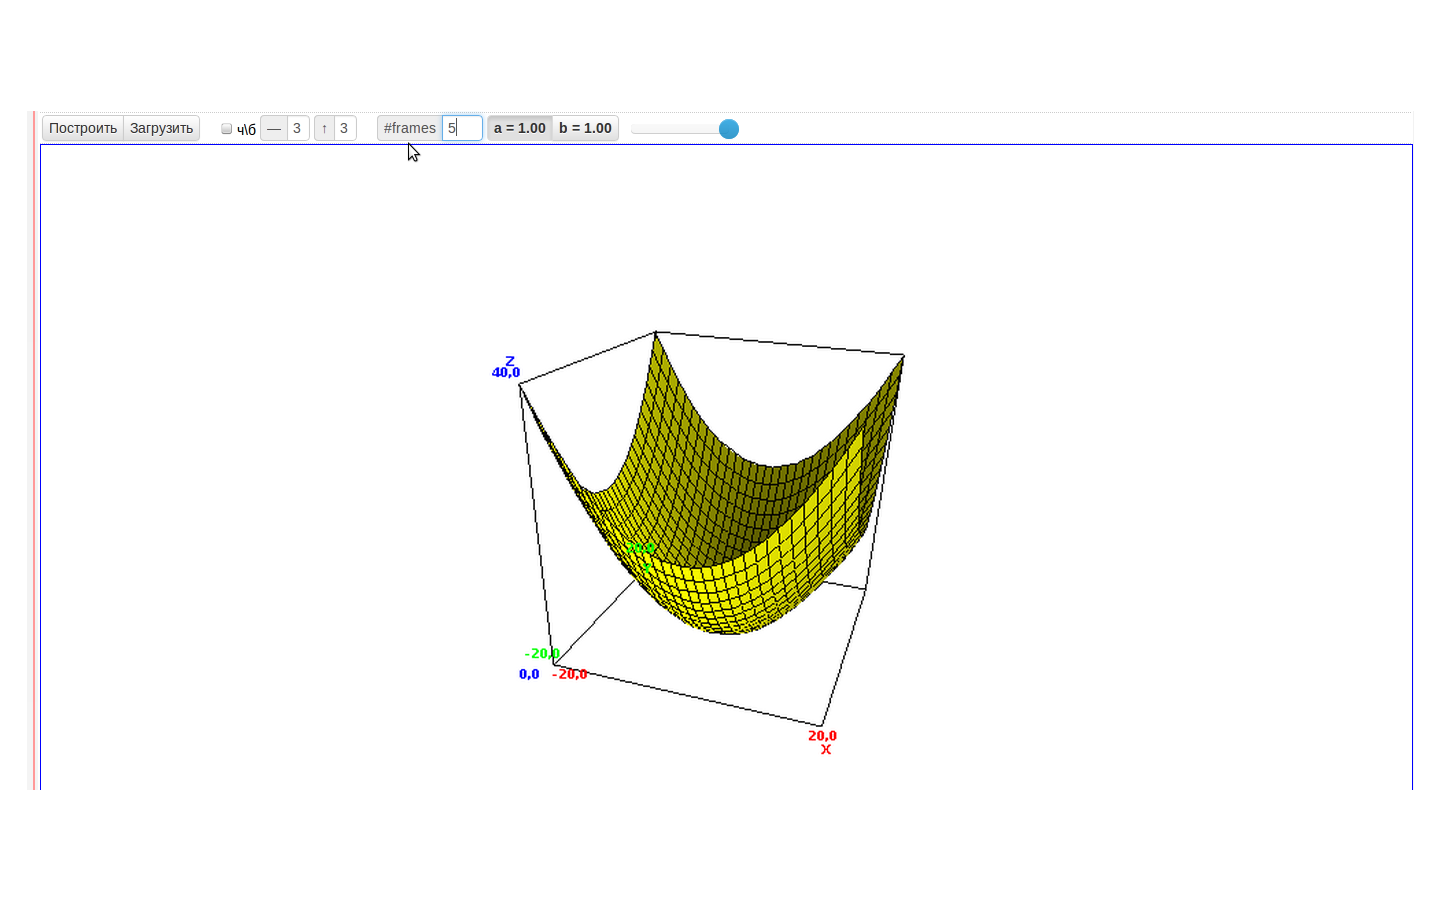
\includegraphics[scale=0.35]{pictures/3_9}
Рис. 1.

Для изменения параметров используйте ползунок - (например установим: a = 0.7, b = 0.24) (см. Рис.2.)

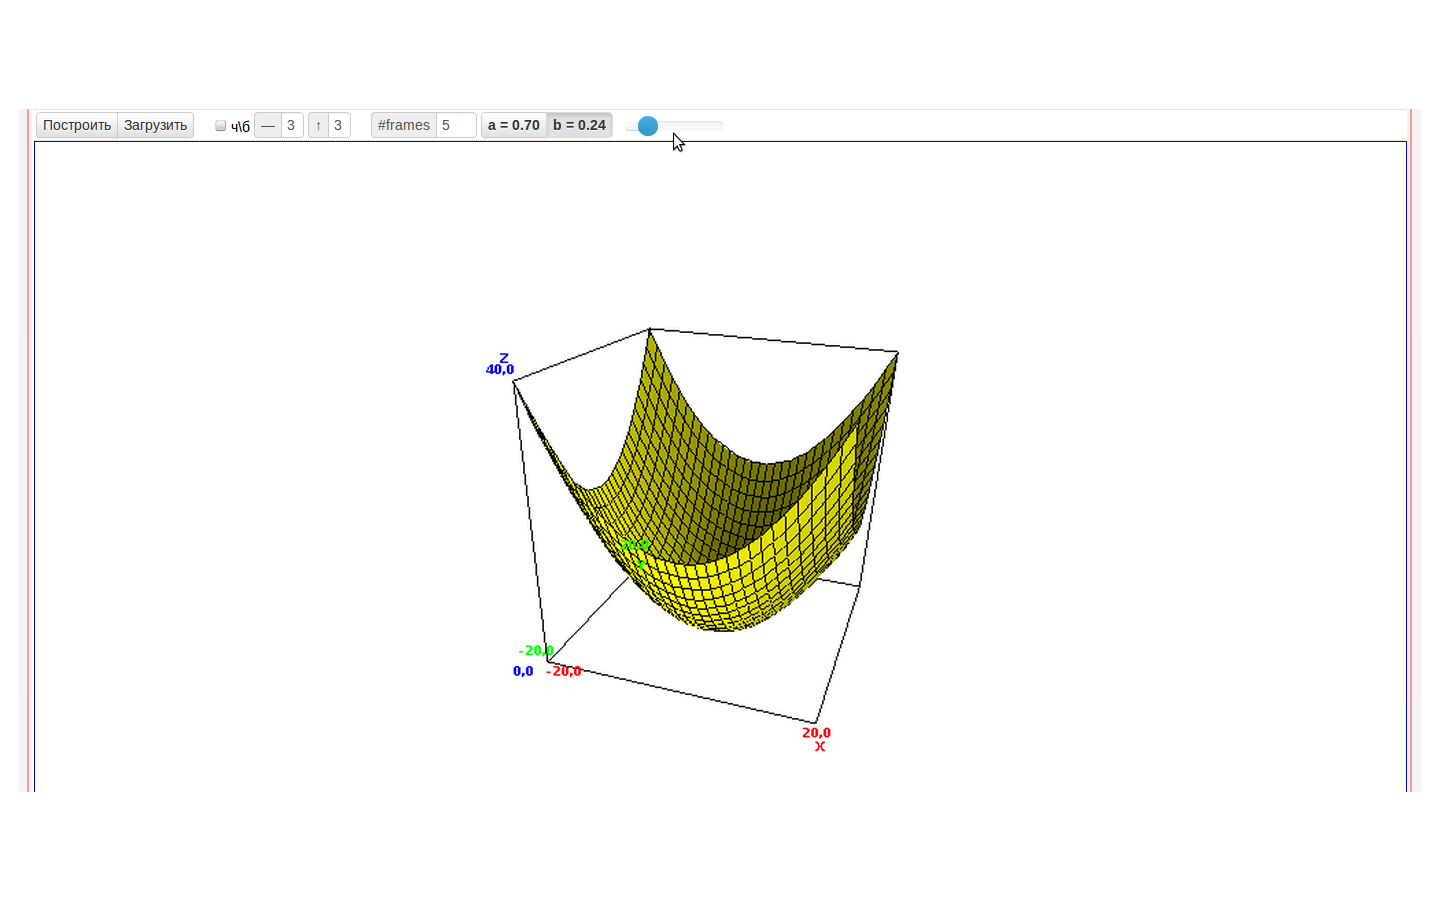
\includegraphics[scale=0.35]{pictures/3_10}
Рис. 2.

Для построения графика нажимаем кнопку - 'Построить' (см. Рис.3.)

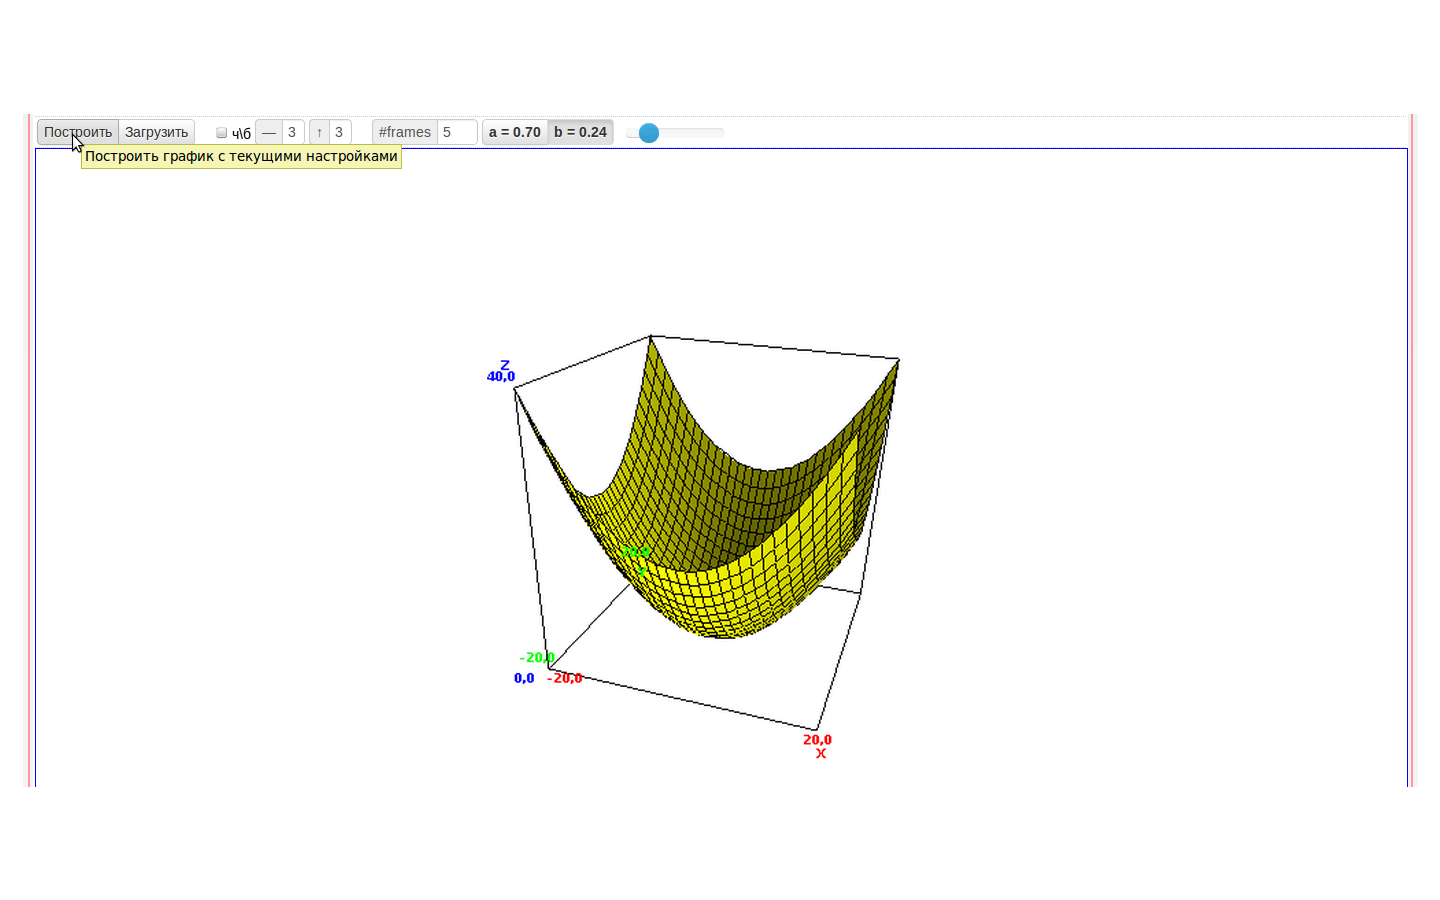
\includegraphics[scale=0.35]{pictures/3_11}
Рис. 3.

В результате получаем график.(см. Рис.4.)

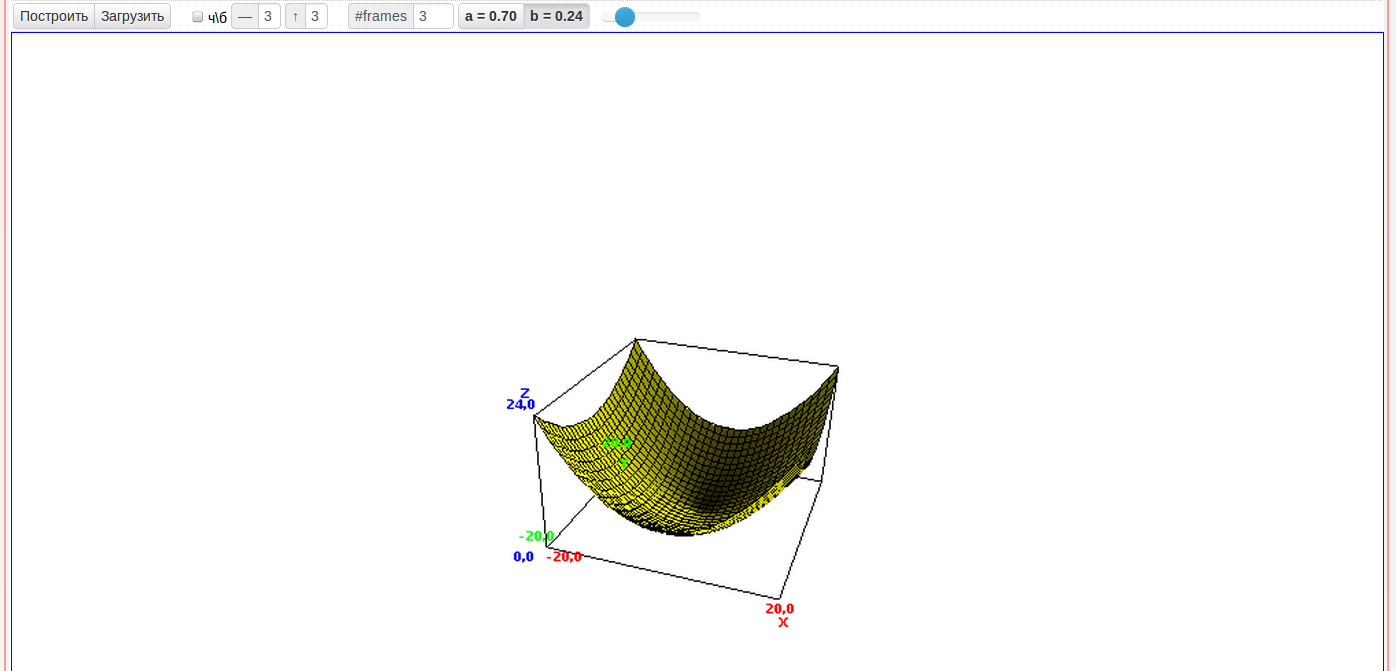
\includegraphics[scale=0.35]{pictures/3_12}
Рис. 4.

%enddelete

%begindelete
 
\ex{$f=x^2/20+y^2/20;$\\
\hspace*{4mm} $plot3d(f, [-20, 20, -20, 20]);$\\
\hspace*{4mm} $plot3d([x/20+y^2/20, x^2/20+y/20], [-20, 20, -20, 20]);$}
{рис. \ref{3_7}.}

\begin{figure}[!ht]
  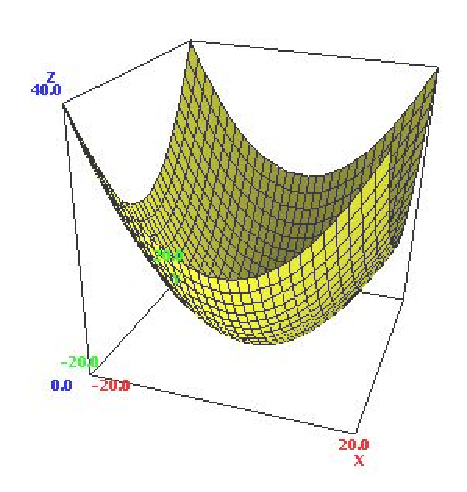
\includegraphics[width=138pt, height=146pt]{pictures/3_7}
  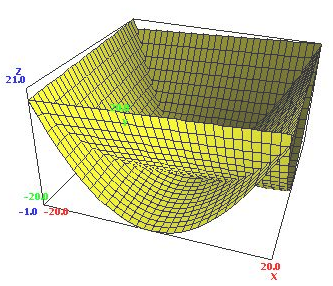
\includegraphics[width=166.5pt, height=143pt]{pictures/3_8}
  \caption{Построение 3D графиков функций}
  \label{3_7}
\end{figure}
%enddelete

Сфера

\begin{verbatim}
SPACE=R64[u,v];
\paramPlot3d([[\cos(u)\cos(v)], [\sin(u)\cos(v)], [\sin(v)]], 
[-\pi, \pi, -\pi/2, \pi/2]);
\end{verbatim}

Тор

\begin{verbatim}
SPACE=R64[u,v];
\paramPlot3d([[\cos(u)(\cos(v)+3)],[\sin(u)(\cos(v)+3)],[\sin(v)]], 
[-\pi, \pi, -\pi, \pi]);
\end{verbatim}

Спираль

\begin{verbatim}
SPACE=R64[u,v];
\paramPlot3d([[\cos(u)(\cos(v)+3)],[\sin(u)(\cos(v)+3)],[\sin(v)+u]], 
[-2\pi, 2\pi, -\pi, \pi]);
\end{verbatim}

Логарифмическая спираль

\begin{verbatim}
SPACE=R64[u,v];
\paramPlot3d([[u\cos(u)(\cos(v)+1)],[u\sin(u)(\cos(v)+1)],[u\sin(v)]], 
[0, 3\pi, -\pi, \pi]);
\end{verbatim}

"Морская раковина"

\begin{verbatim}
SPACE=R64[u,v];
\paramPlot3d([[u\cos(u)(\cos(v)+1)],[u\sin(u)(\cos(v)+1)],
[u\sin(v)-(((u+3)/8)\pi)^2-20]], [0, 8\pi, -\pi, \pi]);
\end{verbatim}

Трилистник

\begin{verbatim}
SPACE=R64[u,v];
\paramPlot3d([[\cos(u)\cos(v)+3\cos(u)(1.5+\sin(1.5u/2))],
[\sin(u)\cos(v)+3\sin(u)(1.5+\sin(1.5u/2))],[\sin(v)+2\cos(1.5u)]], 
[-2\pi, 2\pi, -\pi, \pi]);
\end{verbatim}

Поверхность Дини

\begin{verbatim}
SPACE=R64[u,v];
\paramPlot3d([[\cos(u)\sin(v)],[\sin(u)\sin(v)],
[\cos(v)+\lg(\tg(v/2))+0.2u-4]], [0, 4\pi, 0.0001, 2]);
\end{verbatim}

Лента Мёбиуса

\begin{verbatim}
SPACE=R64[u,v];
\paramPlot3d([[(1+v/2\cos(u/2))\cos(u)],[(1+v/2\cos(u/2))\sin(u)],
[v/2\sin(u/2)]], [0, 2\pi, -1, 1]);
\end{verbatim}

Куб

\begin{verbatim}
SPACE=R64[u,v];
\paramPlot3d([[u,v,5,u,v,-5],[v,5,u,v,-5,u],[5,u,v,-5,u,v]], 
[-5, 5, -5, 5]);
\end{verbatim}

Цилиндр

\begin{verbatim}
SPACE=R64[u,v];
\paramPlot3d([[5\cos(u)],[5\sin(u)],[v]], [-5, 5, -5, 5]);
\end{verbatim}

Конус

\begin{verbatim}
SPACE=R64[u,v];
\paramPlot3d([[\cos(u) * (5 * (1 - v/6))],[\sin(u) * (5 * (1 - v/6))],[v]], 
[-6, 6, 0, 6]);
\end{verbatim}

Усеченный конус

\begin{verbatim}
SPACE=R64[u,v];
\paramPlot3d([[\cos(u) * (5 * (1 - v/6) + 1 * v/6)],
[\sin(u) * (5 * (1 - v/6) + 1 * v/6) ],[v]], [-5, 5, -5, 5]);
\end{verbatim}

Песочные часы

\begin{verbatim}
SPACE=R64[u,v];
\paramPlot3d([[\cos(u) * (5 * (0.5 - v/6) + 0.01*v/6)],
[\sin(u) * (5 * (0.5 - v/6) + 0.01*v/6)],[v]], [0, 2\pi, 0, 2\pi]);
\end{verbatim}



\section{Построение 3D графиков  функций, которые заданы неявно}
 Mathpar позволяет строить 3D графики неявно заданных функций. 
 
 Для построения  графика функции $f(x,y,z)=0$ используется команда 
 
\comm{implicitPlot3d}{(f, xMin, xMax, yMin, yMax, zMin, zMax)}, 

где числа $xMin, xMax, yMin, yMax, zMin, zMax$ задают область в пространстве, имеющую форму параллелепипеда,
в которой изображается неявная функция. 

Можно задавать только одну функцию, следующим образом:

\comm{implicitPlot3d}{(f)},

в этом случае предполагается, что будет изображена функция $f$ в кубе $20\times20\times20$, 
центр которого распологается в начале координат.

Вы можете вращать систему координат перемещая указатель мышки с нажатой левой клавишей. 
Вы можете сдвигать начало системы координат перемещая указатель мышки с нажатой правой клавишей. 

Moжно, дополнительно, указывать координаты источника света, цвет и сетку. По умолчанию принимается
сетка из 50 точек на кажом ребре параллелепипеда. 

Цвет в формате RGB (красный, зеленый, голубой) задается числом

$R*256*256+G*256+B$,

 где каждая буква обозначает неотрицательное целое число не превосходящее 255.
Например, $255*256*256$ -- красный цвет, а $255*256*256+ 255*256$ -- желтый (красный+зеленый).
Допускаются, кроме того, следующие наборы аргументов: 

$(f,xMin, xMax, yMin, yMax, zMin, zMax, gridSize)$,

$(f,xMin, xMax, yMin, yMax, zMin, zMax, lightX, lightY, lightZ, gridSize )$,

$(f,xMin, xMax, yMin, yMax, zMin, zMax, lightX, lightY, lightZ, color, gridSize)$.

%begindelete
\underline{Example. }

\vspace*{-2mm}
%enddelete


\begin{verbatim}
SPACE = R64[x, y, z];
f = -x^2+2y^2+3z^2-25;
\implicitPlot3d( f, -10, 10, -10, 10, -10, 10);
\end{verbatim}

Гиперболоид

\begin{verbatim}
SPACE = R64[x, y, z ];
\implicitPlot3d( x^2+ y^2+ z^2-25 , -7, 7, -7, 7, -7, 7,10, 10, 10, 255*256*256, 100);
\end{verbatim}

Красная сфера 




\begin{verbatim}
SPACE = R64[x, y, z]; 
f =  \sin(xyz/100) ;
\implicitPlot3d( f , -9,9,-9,9,-9,9, 10,10,4, 255*256*256+255*256, 50);
\end{verbatim}

Желтая поверхность с центральной симметрией.

\begin{verbatim}
SPACE = R64[x, y, z]; 
f = ((x+2)^2+ (y-2)^2 -1)((x-2)^2+ (y+2)^2 -1)((x+2)^2+ (y+2)^2 -1) ((x-2)^2+ (y-2)^2 -1)(x^2+ y^2 -1); 
\implicitPlot3d( f, -10, 10, -10, 10, -10, 10 );
\end{verbatim}


Органные трубы.


%begindelete
\section{Контрольные задания}
В Mathpar постройте графики функций
\begin{itemize}
 \item $f(x)=x^2+2y, $
 \item $f(x)=\sqrt{\sin ^2(5x-1)+\exp x}, $
 \item $f(x, y) = \sin(\cos(x+\tan(y))). $
\end{itemize}
%enddelete

